\chapter{Drawing conclusions}
\label{ch:grand-finale}

\section{The main equivalence}
In general, we can define a monoidal functor by just evaluating it on the generators of the source category.
In our case, where a two-dimensional TQFT is a symmetric monoidal functor $Z \colon \bord{2} \to \mathbf{Vect}_\Bbbk$, this implies that $Z$ is entirely described by its evaluation on the generating morphisms (and the objects of the skeleton).

Following the definition of a TQFT we then choose a $\Bbbk$-vector space $A$ as the image of the circle
\[
 (\mathbf{1}) \mapsto A
\]
and, by functoriality,
\[
 \bordcylinder \mapsto [\id_A \colon A \to A]
\]
Being $Z$ a symmetric monoidal functor, it also follows that
\[
 (\mathbf{n}) \mapsto A \tensor \dots \tensor A = A^{\tensor n}
 \hspace{3em}\text{and}\hspace{3em}
 \bordtwist \mapsto [\sigma\colon A \tensor A \to A \tensor A]
\]
The images of the remaining generators are defined as follows
\begin{align*}
 \bordcap     & \mapsto [\eta \colon \Bbbk \to A] \hspace{3.5em} \wireunit          \\
 \bordpants   & \mapsto [\mu \colon A \tensor A \to A] \hspace{1em} \wiremult       \\
 \bordcocap   & \mapsto [\varepsilon \colon A \to \Bbbk] \hspace{3.5em} \wirecounit \\
 \bordcopants & \mapsto [\delta \colon A \to A \tensor A] \hspace{1em} \wirecomult
\end{align*}
The relations in $\bord{2}$ then become relations between these $\Bbbk$-linear maps. For example, for the handle cancellation, we have:
\[
 \begin{tikzpicture}[every tqft/.style={transform shape, bottom color=gray, top color=white, fill opacity=0.5}, tqft/view from=incoming, tqft/boundary separation=1.5cm, rotate=-90, scale=0.4, baseline=-2pt]
  \pic[tqft pair of pants, name=a, draw,
   every incoming lower boundary component/.style={draw},
   anchor=incoming boundary 1,
   every incoming boundary component/.style={fill=gray, fill opacity=0.7}];
  \pic[tqft cup, anchor=incoming boundary 1, name=b, at=(a-outgoing boundary 1), draw, every lower boundary component/.style={dashed, draw}];
  \pic[tqft cylinder, anchor=incoming boundary 1, name=c, at=(a-outgoing boundary 2), draw, every lower boundary component/.style={dashed, draw}];
 \end{tikzpicture}
 =
 \begin{tikzpicture}[every tqft/.style={transform shape, bottom color=gray, top color=white, fill opacity=0.5}, tqft/view from=incoming, tqft/boundary separation=1.5cm, rotate=-90, scale=0.4, baseline=-2pt]
  \pic[tqft cylinder, name=a, draw, every incoming lower boundary component/.style={draw}, every outgoing lower boundary component/.style={dashed, draw}, anchor=outgoing boundary 1, every incoming boundary component/.style={fill=gray, fill opacity=0.7}];
 \end{tikzpicture}
 =
 \begin{tikzpicture}[every tqft/.style={transform shape, bottom color=gray, top color=white, fill opacity=0.5}, tqft/view from=incoming, tqft/boundary separation=1.5cm, rotate=-90, scale=0.4, baseline=-2pt]
  \pic[tqft pair of pants, name=a, draw, every incoming lower boundary component/.style={draw}, anchor=incoming boundary 1, every incoming boundary component/.style={fill=gray, fill opacity=0.7}];
  \pic[tqft cup, anchor=incoming boundary 1, name=b, at=(a-outgoing boundary 2), draw, every lower boundary component/.style={dashed, draw}];
  \pic[tqft cylinder, anchor=incoming boundary 1, name=c, at=(a-outgoing boundary 1), draw, every lower boundary component/.style={dashed, draw}];
 \end{tikzpicture}
 \hspace{1em}\text{becomes}\hspace{1em}
 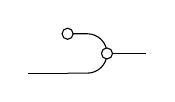
\begin{tikzpicture}[x=0.5cm, y=0.25cm, baseline]
  \draw[rounded corners=0.25cm] (-1,1) -- (0,1) -- (0,0);
  \draw[rounded corners=0.25cm] (-1,-1) -- (0,-1) -- (0,0);
  \draw (-1,-1) -- (-2,-1);
  \draw (0,0) -- (1,0);
  \draw[fill=white] (0,0) circle (2pt);
  \draw[fill=white] (-1,1) circle (2pt);
 \end{tikzpicture}
 \:=\:
 \begin{tikzpicture}[x=0.5cm, y=0.25cm, baseline]
  \draw (0,0) -- (1,0);
 \end{tikzpicture}
 \:=\:
 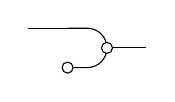
\begin{tikzpicture}[x=0.5cm, y=0.25cm, baseline]
  \draw[rounded corners=0.25cm] (-1,1) -- (0,1) -- (0,0);
  \draw[rounded corners=0.25cm] (-1,-1) -- (0,-1) -- (0,0);
  \draw (-1,1) -- (-2,1);
  \draw (0,0) -- (1,0);
  \draw[fill=white] (0,0) circle (2pt);
  \draw[fill=white] (-1,-1) circle (2pt);
 \end{tikzpicture}
\]

By ``slimming'' all the relations in $\bord{2}$, it should becomes obvious there exists some kind of relation between topological quantum field theories and the Frobenius structure we studied in the previous chapter.
These considerations lead us to the main theorem regarding the classification of 2-dimensional TQFTs.
\begin{tcbthm} \label{thm:equiv}
 There is a canonical equivalence of categories between 2-dimensional TQFTs taking values in $\mathbf{Vect}_\Bbbk$ and commutative Frobenius $\Bbbk$-algebras.\index{$\mathbf{2TQFT}_\Bbbk$, a category of two dimensional TQFTs}\index{$\mathbf{cFAlg}_\Bbbk$, a category of commutative Frobenius algebras}
 \[
  \mathbf{2TQFT}_\Bbbk \iso \mathbf{cFAlg}_\Bbbk
 \]
\end{tcbthm}

Thanks to our journey through the previous chapters the proof becomes straightforward. We can now explicitly bulid the correspondence, for both objects and arrows.

Indeed, given an object $Z$ in $\textbf{2TQFT}_\Bbbk$ we get the axioms defining a structure of commutative Frobenius algebra on the vector space $Z((\mathbf{1})) = A$.

\[
 \begin{tikzpicture}[every tqft/.style={transform shape, bottom color=gray, top color=white, fill opacity=.5}, tqft/view from=incoming, tqft/boundary separation=1.5cm, rotate=-90, scale=0.4, baseline=-2pt]
  \pic[tqft reverse pair of pants, name=a, draw, every lower boundary component/.style={dashed, draw}, anchor=outgoing boundary 1];
  \pic[tqft cap, anchor=outgoing boundary 1, name=b, at=(a-incoming boundary 1), draw];
  \pic[tqft cylinder, anchor=outgoing boundary 1, name=c, at=(a-incoming boundary 2), draw, every incoming lower boundary component/.style={draw}, every incoming boundary component/.style={fill=gray, fill opacity=0.7}];
 \end{tikzpicture}
 =
 \begin{tikzpicture}[every tqft/.style={transform shape, bottom color=gray, top color=white, fill opacity=0.5}, tqft/view from=incoming, tqft/boundary separation=1.5cm, rotate=-90, scale=0.4, baseline=-2pt]
  \pic[tqft cylinder, name=a, draw, every incoming lower boundary component/.style={draw}, every outgoing lower boundary component/.style={dashed, draw}, anchor=incoming boundary 1, every incoming boundary component/.style={fill=gray, fill opacity=0.7}];
 \end{tikzpicture}
 =
 \begin{tikzpicture}[every tqft/.style={transform shape, bottom color=gray, top color=white, fill opacity=.5}, tqft/view from=incoming, tqft/boundary separation=1.5cm, rotate=-90, scale=0.4, baseline=-2pt]
  \pic[tqft reverse pair of pants, name=a, draw, every lower boundary component/.style={dashed, draw}, anchor=outgoing boundary 1];
  \pic[tqft cap, anchor=outgoing boundary 1, name=b, at=(a-incoming boundary 2), draw];
  \pic[tqft cylinder, anchor=outgoing boundary 1, name=c, at=(a-incoming boundary 1), draw, every incoming lower boundary component/.style={draw}, every incoming boundary component/.style={fill=gray, fill opacity=0.7}];
 \end{tikzpicture}
 \hspace{1em}\text{becomes}\hspace{1em}
 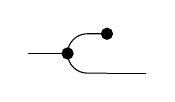
\begin{tikzpicture}[x=0.5cm, y=0.25cm, baseline]
  \draw[rounded corners=0.25cm] (1,1) -- (0,1) -- (0,0);
  \draw[rounded corners=0.25cm] (1,-1) -- (0,-1) -- (0,0);
  \draw (1,-1) -- (2,-1);
  \draw (0,0) -- (-1,0);
  \draw[fill=black] (0,0) circle (2pt);
  \draw[fill=black] (1,1) circle (2pt);
 \end{tikzpicture}
 \:=\:
 \begin{tikzpicture}[x=0.5cm, y=0.25cm, baseline]
  \draw (0,0) -- (1,0);
 \end{tikzpicture}
 \:=\:
 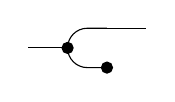
\begin{tikzpicture}[x=0.5cm, y=0.25cm, baseline]
  \draw[rounded corners=0.25cm] (1,1) -- (0,1) -- (0,0);
  \draw[rounded corners=0.25cm] (1,-1) -- (0,-1) -- (0,0);
  \draw (1,1) -- (2,1);
  \draw (0,0) -- (-1,0);
  \draw[fill=black] (0,0) circle (2pt);
  \draw[fill=black] (1,-1) circle (2pt);
 \end{tikzpicture}
\]

\[
 \begin{tikzpicture}[every tqft/.style={transform shape, bottom color=gray, top color=white, fill opacity=0.5}, tqft/view from=incoming, tqft/boundary separation=1.5cm, rotate=-90, scale=0.4, baseline=-2pt]
  \pic[tqft pair of pants, name=a, draw, anchor=outgoing boundary 1,
   every incoming lower boundary component/.style={draw},
   every incoming boundary component/.style={fill=gray, fill opacity=0.7}];
  \pic[tqft reverse pair of pants, name=b, draw, anchor=incoming boundary 2, at=(a-outgoing boundary 1),
   every lower boundary component/.style={dashed, draw}];
  \pic[tqft cylinder to prior, draw, anchor=incoming boundary, at=(a-outgoing boundary 2),
   every lower boundary component/.style={dashed, draw}];
  \pic[tqft cylinder to prior, draw, anchor=outgoing boundary, at=(b-incoming boundary 1),
   every incoming lower boundary component/.style={draw},
   every incoming boundary component/.style={fill=gray, fill opacity=0.7}];
 \end{tikzpicture}
 =
 \begin{tikzpicture}[every tqft/.style={transform shape, bottom color=gray, top color=white, fill opacity=0.5}, tqft/view from=incoming, tqft/boundary separation=1.5cm, rotate=-90, scale=0.4, baseline=-2pt]
  \pic[tqft pair of pants, name=a, draw,
   every lower boundary component/.style={dashed, draw}];
  \pic[tqft reverse pair of pants, draw, anchor=outgoing boundary, at=(a-incoming boundary),
   every incoming lower boundary component/.style={draw},
   every incoming boundary component/.style={fill=gray, fill opacity=0.7}];
 \end{tikzpicture}
 =
 \begin{tikzpicture}[every tqft/.style={transform shape, bottom color=gray, top color=white, fill opacity=0.5}, tqft/view from=incoming, tqft/boundary separation=1.5cm, rotate=-90, scale=0.4, baseline=-2pt]
  \pic[tqft pair of pants, name=a, draw, anchor=outgoing boundary 2,
   every incoming lower boundary component/.style={draw},
   every incoming boundary component/.style={fill=gray, fill opacity=0.7}];
  \pic[tqft reverse pair of pants, name=b, draw, anchor=incoming boundary 1, at=(a-outgoing boundary 2),
   every lower boundary component/.style={dashed, draw}];
  \pic[tqft cylinder to next, draw, anchor=incoming boundary, at=(a-outgoing boundary 1),
   every lower boundary component/.style={dashed, draw}];
  \pic[tqft cylinder to next, draw, anchor=outgoing boundary, at=(b-incoming boundary 2),
   every incoming lower boundary component/.style={draw},
   every incoming boundary component/.style={fill=gray, fill opacity=0.7}];
 \end{tikzpicture}
 \hspace{1em}\text{becomes}\hspace{.5em}
 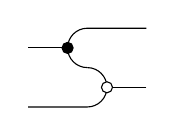
\begin{tikzpicture}[x=0.5cm, y=0.25cm, baseline,yshift=-0.25cm]
  \draw[rounded corners=0.25cm] (0,2) -- (0,1) -- (.5,1);
  \draw[rounded corners=0.25cm] (0,2) -- (0,3) -- (2,3);
  \draw[rounded corners=0.25cm] (1,0) -- (1,1) -- (.5,1);
  \draw[rounded corners=0.25cm] (1,0) -- (1,-1) -- (-1,-1);
  \draw (2,0)--(1,0);
  \draw (0,2)--(-1,2);
  \draw[fill=black] (0,2) circle (2pt);
  \draw[fill=white] (1,0) circle (2pt);
 \end{tikzpicture}
 \:=\:
 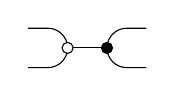
\begin{tikzpicture}[x=0.5cm, y=0.25cm, baseline]
  \draw[rounded corners=0.25cm] (-1,-1) -- (0,-1) -- (0,0);
  \draw[rounded corners=0.25cm] (-1,1) -- (0,1) -- (0,0);
  \draw (0,0) -- (1,0);
  \draw[fill=white] (0,0) circle (2pt);
  \draw[fill=black] (1,0) circle (2pt);
  \draw[rounded corners=0.25cm] (1,0) -- (1,1) -- (2,1);
  \draw[rounded corners=0.25cm] (1,0) -- (1,-1) -- (2,-1);
 \end{tikzpicture}
 \:=\:
 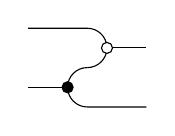
\begin{tikzpicture}[x=0.5cm, y=0.25cm, baseline,yshift=-0.25cm]
  \draw[rounded corners=0.25cm] (0,2) -- (0,1) -- (-.5,1);
  \draw[rounded corners=0.25cm] (0,2) -- (0,3) -- (-2,3);
  \draw[rounded corners=0.25cm] (-1,0) -- (-1,1) -- (-.5,1);
  \draw[rounded corners=0.25cm] (-1,0) -- (-1,-1) -- (1,-1);
  \draw (-2,0)--(-1,0);
  \draw (0,2)--(1,2);
  \draw[fill=white] (0,2) circle (2pt);
  \draw[fill=black] (-1,0) circle (2pt);
 \end{tikzpicture}
\]

\[
 \begin{tikzpicture}[every tqft/.style={transform shape, bottom color=gray, top color=white, fill opacity=0.5}, tqft/view from=incoming, rotate=-90, scale=0.4, baseline=-2pt]
  \pic[tqft pair of pants, draw, name=a,
   boundary separation=1.5cm,
   every incoming lower boundary component/.style={draw},
   every incoming boundary component/.style={fill=gray, fill opacity=0.7}];
  \pic[tqft,
   incoming boundary components=1,
   outgoing boundary components=1,
   offset=-.75,
   anchor=incoming boundary,
   at=(a-outgoing boundary 2),
   draw,
   every lower boundary component/.style={dashed, draw}];
  \pic[tqft,
   incoming boundary components=1,
   outgoing boundary components=1,
   offset=.75,
   anchor=incoming boundary,
   at=(a-outgoing boundary 1),
   draw,
   every lower boundary component/.style={dashed, draw}];
 \end{tikzpicture}
 =
 \begin{tikzpicture}[every tqft/.style={transform shape, bottom color=gray, top color=white, fill opacity=0.5}, tqft/view from=incoming, rotate=-90, scale=0.4, baseline=-2pt]
  \pic[tqft pair of pants, draw, name=a,
   boundary separation=1.5cm,
   every incoming lower boundary component/.style={draw},
   every incoming boundary component/.style={fill=gray, fill opacity=0.7},
   every outgoing lower boundary component/.style={dashed, draw}];
 \end{tikzpicture}
 \hspace{1em}\text{becomes}\hspace{1em}
 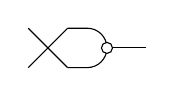
\begin{tikzpicture}[x=0.5cm, y=0.25cm, baseline]
  \draw[rounded corners=0.25cm] (-1,1) -- (0,1) -- (0,0);
  \draw[rounded corners=0.25cm] (-1,-1) -- (0,-1) -- (0,0);
  \draw (0,0) -- (1,0);
  \draw (-2,-1) -- (-1,1);
  \draw (-2,1) -- (-1,-1);
  \draw[fill=white] (0,0) circle (2pt);
 \end{tikzpicture}
 \:=\:
 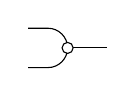
\begin{tikzpicture}[x=0.5cm, y=0.25cm, baseline]
  \draw[rounded corners=0.25cm] (-1,1) -- (0,1) -- (0,0);
  \draw[rounded corners=0.25cm] (-1,-1) -- (0,-1) -- (0,0);
  \draw (0,0) -- (1,0);
  \draw[fill=white] (0,0) circle (2pt);
 \end{tikzpicture}
\]
\[
 \begin{tikzpicture}[every tqft/.style={transform shape, bottom color=gray, top color=white, fill opacity=0.5}, tqft/view from=incoming, rotate=-90, scale=0.4, baseline=-2pt]
  \pic[tqft reverse pair of pants, anchor=outgoing boundary, draw, name=a,
   boundary separation=1.5cm,
   every lower boundary component/.style={dashed, draw}];
  \pic[tqft,
   incoming boundary components=1,
   outgoing boundary components=1,
   offset=-.75,
   anchor=outgoing boundary,
   at=(a-incoming boundary 1),
   draw,
   every incoming lower boundary component/.style={draw},
   every incoming boundary component/.style={fill=gray, fill opacity=0.7},
   every outgoing lower boundary component/.style={dashed, draw}];
  \pic[tqft,
   incoming boundary components=1,
   outgoing boundary components=1,
   offset=.75,
   anchor=outgoing boundary,
   at=(a-incoming boundary 2),
   draw,
   every incoming lower boundary component/.style={draw},
   every incoming boundary component/.style={fill=gray, fill opacity=0.7},
   every outgoing lower boundary component/.style={dashed, draw}];
 \end{tikzpicture}
 =
 \begin{tikzpicture}[every tqft/.style={transform shape, bottom color=gray, top color=white, fill opacity=0.5}, tqft/view from=incoming, rotate=-90, scale=0.4, baseline=-2pt]
  \pic[tqft reverse pair of pants, anchor=outgoing boundary, draw, name=a,
   boundary separation=1.5cm,
   every incoming lower boundary component/.style={draw},
   every incoming boundary component/.style={fill=gray, fill opacity=0.7},
   every outgoing lower boundary component/.style={dashed, draw}];
 \end{tikzpicture}
 \hspace{1em}\text{becomes}\hspace{1em}
 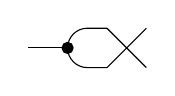
\begin{tikzpicture}[x=0.5cm, y=0.25cm, baseline]
  \draw[rounded corners=0.25cm] (0,0) -- (0,1) -- (1,1);
  \draw[rounded corners=0.25cm] (0,0) -- (0,-1) -- (1,-1);
  \draw (-1,0)--(0,0);
  \draw (1,1)--(2,-1);
  \draw (1,-1)--(2,1);
  \draw[fill=black] (0,0) circle (2pt);
 \end{tikzpicture}
 \:=\:
 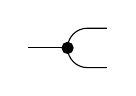
\begin{tikzpicture}[x=0.5cm, y=0.25cm, baseline]
  \draw[rounded corners=0.25cm] (0,0) -- (0,1) -- (1,1);
  \draw[rounded corners=0.25cm] (0,0) -- (0,-1) -- (1,-1);
  \draw (-1,0)--(0,0);
  \draw[fill=black] (0,0) circle (2pt);
 \end{tikzpicture}
\]

Conversely, given a commutative Frobenius algebra $(A, \eta, \mu, \varepsilon, \delta)$, we are able to determine a TQFT by evaluation on the generating morphisms as described above.

These assignments define a bijection. Starting with a symmetric monoidal functor $Z$ we obtain a commutative Frobenius algebra $A = Z((\mathbf{1}))$. From such algebra we then define a TQFT by mapping $(\mathbf{1})$ onto it, which exactly corresponds to the monoidal functor we started with.

To check this defines an equivalence between the two categories we must also consider what happens to morphisms. By definition, an arrow $u \colon Z \to Z'$ between two 2-dimensional TQFTs is a monoidal natural transformations between the two functors. In particular, the structure of $\bord{2}$, implies that these natural transformations consist of $\Bbbk$-linear maps $A^{\tensor n} \to A'^{\tensor n}$, where $A = Z((\mathbf{1}))$, $A' = Z'((\mathbf{1}))$, compatible with all the arrows in $\bord{2}$. Furthermore, by asking $u$ to be monoidal, these arrows are just the $n$-th tensor power of the $\Bbbk$-linear arrow $u_1 \colon A \to A'$.
Since every arrow in $\bord{2}$ is built by tesoring and gluing the generators, the compatibility of $u$ with the arrows in $\bord{2}$ is entirly determined by the corresponding diagrams.

\[
 \begin{tikzcd}
  \Bbbk \arrow[r, equal] \arrow[d, "\eta"] & \Bbbk \arrow[d, "\eta'"] \\
  A \arrow[r, "u_1"] & A'
 \end{tikzcd}
 \hspace{3em}
 \begin{tikzcd}[column sep=5em]
  A \tensor A \arrow[r, "u_1 \tensor u_1"] \arrow[d, "\mu"] & A' \tensor A' \arrow[d, "\mu'"]\\
  A \arrow[r, "u_1"] & A'
 \end{tikzcd}
\]
\[
 \begin{tikzcd}
  A \arrow[r, "u_1"] \arrow[d, "\varepsilon"] & A' \arrow[d, "\varepsilon'"] \\
  \Bbbk \arrow[r, equal] & \Bbbk
 \end{tikzcd}
 \hspace{3em}
 \begin{tikzcd}[column sep=5em]
  A \arrow[r, "u_1"] \arrow[d, "\delta"] & A' \arrow[d, "\delta'"] \\
  A \tensor A' \arrow[r, "u_1 \tensor u_1"] & A'\tensor A'
 \end{tikzcd}
\]
\[
 \begin{tikzcd}[column sep=5em]
  A \tensor A \arrow[r, "u_1 \tensor u_1" ] \arrow[d, "\sigma"] & A' \tensor A' \arrow[d, "\sigma'"] \\
  A \tensor A \arrow[r, "u_1 \tensor u_1"] & A'\tensor A'
 \end{tikzcd}
\]

Let us now go back to the definitions of algebra and coalgebra homomorphisms.\todo{add ref} We notice that the commutative diagrams there are formally identical to the naturality condition imposed on the monoidal transformation $u \colon Z \to Z'$. We then have proved that each monoidal transformation in $\bord{2}$ defines a morphism of Frobenius algebras, hence (by symmetry of the functors $Z$ and $Z'$) of commutative ones.

By applying the same argument backwards we reach the converse implication, thus completing the proof of the categorical equivalence.


\section{A broader result}

\todo[inline]{Let us put everything in the right context...}


\begin{tcbdfn}[Internal monoids]
 \label{dfn:internal-monoid}
 Let $(\cat{C}, \sq, I)$ be a monoidal category. An \emph{internal comonoid}\index{internal monoid} in $\cat{C}$ is an object $M$ equipped with two morphisms
 \[
  \mu \colon M \sq M \to M \quad\text{(multiplication)}
  \hspace{3em}
  \eta \colon I \to M \quad\text{(unit)}
 \]
 such that the following diagrams commute
 \[
  \begin{tikzcd}
   & M \sq M \sq M \arrow[dr, "\id_M \sq \mu"] \arrow[dl, "\mu \sq \id_M", swap] & \\
   M \sq M \arrow[dr, "\mu", swap] & & M \sq M \arrow[dl, "\mu"] \\
   & M &
  \end{tikzcd}
 \]
 \[
  \begin{tikzcd}
   & M \sq M \arrow[rd, "\mu"] & & M \sq M \arrow[ld, "\mu", swap]& \\
   I \sq M \arrow[ru, "\eta \sq \id_M"] \arrow[rr, "=", swap]& & M & & M \sq I \arrow[lu, "\id_M \sq \eta", swap] \arrow[ll, "="]
  \end{tikzcd}
 \]
\end{tcbdfn}

The attentive reader has surely noticed that this definition is given on a strict monoidal category. The reason behind this choice is again \ref{thm:strictification}. The general definition is not so different, we report it below for completeness\footnote{And also because in categories like $(\mathbf{Cat}, \times, \mathbf{1})$, $(\mathbf{Vect}_\Bbbk, \tensor, \Bbbk)$ we do not actually have strict unitality.}.

\begin{dfnx*}[Internal monoids]
 Let $(\cat{C}, \sq, I, \alpha, l, r)$ be a monoidal category. An \emph{internal monoid} in $\cat{C}$ is an object $M$ together with two morphisms
 \[
  \mu \colon M \sq M \to M \quad \text{(multiplication)}
  \hspace{3em}
  \eta \colon I \to M \quad \text{(unit)}
 \]
 such that the following diagrams commute
 \[
  \begin{tikzcd}[row sep=2em]
   (M \sq M) \sq M \arrow[rr, "\alpha"] \arrow[d, "\mu \sq \id_M"] & & M \sq (M \sq M) \arrow[d, "\id_M \sq \mu"] \\
   M \sq M \arrow[dr, "\mu", swap] & & M \sq M \arrow[dl, "\mu"] \\
   & M &
  \end{tikzcd}
 \]
 \[
  \begin{tikzcd}
   & M \sq M \arrow[rd, "\mu"] & & M \sq M \arrow[ld, "\mu", swap]& \\
   I \sq M \arrow[ru, "\eta \sq \id_M"] \arrow[rr, "l_M", swap]& & M & & M \sq I \arrow[lu, "\id_M \sq \eta", swap] \arrow[ll,"r_M"]
  \end{tikzcd}
 \]
\end{dfnx*}

By reversing the arrows, we also give the definition of \emph{internal comonoid}.

\begin{tcbdfn}[Internal comonoids]
 \label{dfn:internal-comonoid}
 Let $(\cat{C}, \sq, I)$ be a monoidal category. An \emph{internal comonoid}\index{internal comonoid} in $\cat{C}$ is an object $M$ equipped with two morphisms
 \[
  \delta \colon M \to M \sq M \quad\text{(comultiplication)}
  \hspace{3em}
  \varepsilon \colon M \to I \quad\text{(counit)}
 \]
 such that the following diagrams commute
 \[
  \begin{tikzcd}
   & M \sq M \sq M & \\
   M \sq M \arrow[ur, "\delta \sq \id_M"] & & M \sq M \arrow[ul, "\id_M \sq \delta", swap] \\
   & M \arrow[ul, "\delta"] \arrow[ur, "\delta", swap] &
  \end{tikzcd}
 \]
 \[
  \begin{tikzcd}
   & M \sq M \arrow[dl, "\varepsilon \sq \id_M", swap] & & M \sq M \arrow[dr, "\id_M \sq \varepsilon"]& \\
   I \sq M & & M \arrow[ul, "\delta", swap] \arrow[ur, "\delta"] \arrow[ll, "="] \arrow[rr, "=", swap] & & M
  \end{tikzcd}
 \]
\end{tcbdfn}

Both these structures can be grafically represented, similarly to what we did in the case of $\Bbbk$-Frobenius algebras.

\begin{dfnx*}[Internal monoids]
 Let $(\cat{C}, \sq, I)$ be a monoidal category. An \emph{internal monoid}\index{internal monoid!in terms of wires} in $\cat{C}$ is an object $M$ equipped with two morphisms
 \[
  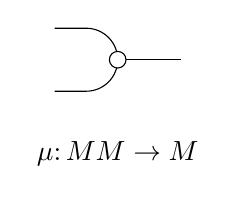
\begin{tikzpicture}[x=0.8cm, y=0.4cm, baseline]
   \draw[rounded corners=0.4cm] (-1,1) -- (0,1) -- (0,0);
   \draw[rounded corners=0.4cm] (-1,-1) -- (0,-1) -- (0,0);
   \draw (0,0) -- (1,0);
   \draw[fill=white] (0,0) circle (3pt);
   \node (mu) at (0,-3) {$\mu \colon M \sq M \to M$};
  \end{tikzpicture}
  \hspace{3em}
  \begin{tikzpicture}[x=0.8cm, y=0.4cm, baseline]
   \draw (0,0)--(1,0);
   \draw[fill=white] (0,0) circle (3pt);
   \node (eta) at (0,-3) {$\eta \colon I \to M$};
  \end{tikzpicture}
 \]
 such that the following relations hold
 \[
  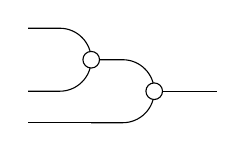
\begin{tikzpicture}[x=0.8cm, y=0.4cm, baseline]
   \draw[rounded corners=0.4cm] (-2,2) -- (-1,2) -- (-1,1);
   \draw[rounded corners=0.4cm] (-2,0) -- (-1,0) -- (-1,1);
   \draw[rounded corners=0.4cm] (-1,1) -- (0,1) -- (0,0);
   \draw[rounded corners=0.4cm] (-1,-1) -- (0,-1) -- (0,0);
   \draw (0,0) -- (1,0);
   \draw (-1,-1) -- (-2,-1);
   \draw[fill=white] (-1,1) circle (3pt);
   \draw[fill=white] (0,0) circle (3pt);
  \end{tikzpicture}
  \quad=\quad
  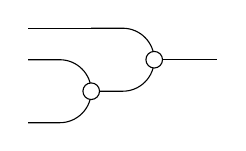
\begin{tikzpicture}[x=0.8cm, y=0.4cm, baseline]
   \draw[rounded corners=0.4cm] (-2,-2) -- (-1,-2) -- (-1,-1);
   \draw[rounded corners=0.4cm] (-2,0) -- (-1,0) -- (-1,-1);
   \draw[rounded corners=0.4cm] (-1,1) -- (0,1) -- (0,0);
   \draw[rounded corners=0.4cm] (-1,-1) -- (0,-1) -- (0,0);
   \draw (0,0) -- (1,0);
   \draw (-1,1) -- (-2,1);
   \draw[fill=white] (-1,-1) circle (3pt);
   \draw[fill=white] (0,0) circle (3pt);
  \end{tikzpicture}
 \]

 \[
  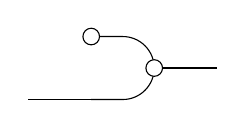
\begin{tikzpicture}[x=0.8cm, y=0.4cm, baseline]
   \draw[rounded corners=0.4cm] (-1,1) -- (0,1) -- (0,0);
   \draw[rounded corners=0.4cm] (-1,-1) -- (0,-1) -- (0,0);
   \draw (-1,-1) -- (-2,-1);
   \draw (0,0) -- (1,0);
   \draw[fill=white] (0,0) circle (3pt);
   \draw[fill=white] (-1,1) circle (3pt);
  \end{tikzpicture}
  \quad=\quad
  \begin{tikzpicture}[x=0.8cm, y=0.4cm, baseline]
   \draw (0,0) -- (1,0);
  \end{tikzpicture}
  \quad=\quad
  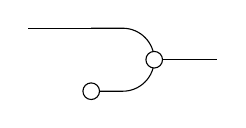
\begin{tikzpicture}[x=0.8cm, y=0.4cm, baseline]
   \draw[rounded corners=0.4cm] (-1,1) -- (0,1) -- (0,0);
   \draw[rounded corners=0.4cm] (-1,-1) -- (0,-1) -- (0,0);
   \draw (-1,1) -- (-2,1);
   \draw (0,0) -- (1,0);
   \draw[fill=white] (0,0) circle (3pt);
   \draw[fill=white] (-1,-1) circle (3pt);
  \end{tikzpicture}
 \]
\end{dfnx*}

\begin{dfnx*}[Internal comonoids]
 Let $(\cat{C}, \sq, I)$ be a monoidal category. An \emph{internal comonoid}\index{internal comonoid!in terms of wires} in $\cat{C}$ is an object $M$ equipped with two morphisms
 \[
  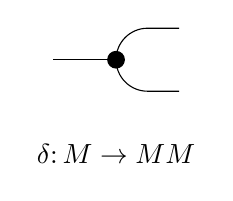
\begin{tikzpicture}[x=0.8cm, y=0.4cm, baseline]
   \draw[rounded corners=0.4cm] (1,1) -- (0,1) -- (0,0);
   \draw[rounded corners=0.4cm] (1,-1) -- (0,-1) -- (0,0);
   \draw (0,0) -- (-1,0);
   \draw[fill=black] (0,0) circle (3pt);
   \node (delta) at (0,-3) {$\delta \colon M \to M \sq M$};
  \end{tikzpicture}
  \hspace{3em}
  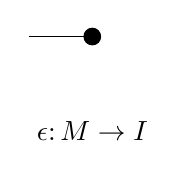
\begin{tikzpicture}[x=0.8cm, y=0.4cm, baseline]
   \draw (0,0)--(-1,0);
   \draw[fill=black] (0,0) circle (3pt);
   \node (epsilon) at (0,-3) {$\epsilon \colon M \to I$};
  \end{tikzpicture}
 \]
 such that the following relations hold
 \[
  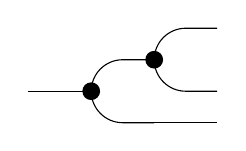
\begin{tikzpicture}[x=0.8cm, y=0.4cm, baseline]
   \draw[rounded corners=0.4cm] (2,2) -- (1,2) -- (1,1);
   \draw[rounded corners=0.4cm] (2,0) -- (1,0) -- (1,1);
   \draw[rounded corners=0.4cm] (1,1) -- (0,1) -- (0,0);
   \draw[rounded corners=0.4cm] (1,-1) -- (0,-1) -- (0,0);
   \draw (0,0) -- (-1,0);
   \draw (1,-1) -- (2,-1);
   \draw[fill=black] (1,1) circle (3pt);
   \draw[fill=black] (0,0) circle (3pt);
  \end{tikzpicture}
  \quad=\quad
  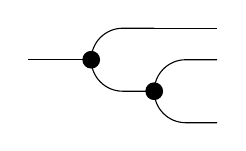
\begin{tikzpicture}[x=0.8cm, y=0.4cm, baseline]
   \draw[rounded corners=0.4cm] (2,-2) -- (1,-2) -- (1,-1);
   \draw[rounded corners=0.4cm] (2,0) -- (1,0) -- (1,-1);
   \draw[rounded corners=0.4cm] (1,1) -- (0,1) -- (0,0);
   \draw[rounded corners=0.4cm] (1,-1) -- (0,-1) -- (0,0);
   \draw (0,0) -- (-1,0);
   \draw (1,1) -- (2,1);
   \draw[fill=black] (1,-1) circle (3pt);
   \draw[fill=black] (0,0) circle (3pt);
  \end{tikzpicture}
 \]

 \[
  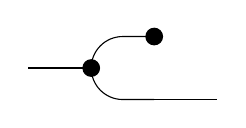
\begin{tikzpicture}[x=0.8cm, y=0.4cm, baseline]
   \draw[rounded corners=0.4cm] (1,1) -- (0,1) -- (0,0);
   \draw[rounded corners=0.4cm] (1,-1) -- (0,-1) -- (0,0);
   \draw (1,-1) -- (2,-1);
   \draw (0,0) -- (-1,0);
   \draw[fill=black] (0,0) circle (3pt);
   \draw[fill=black] (1,1) circle (3pt);
  \end{tikzpicture}
  \quad=\quad
  \begin{tikzpicture}[x=0.8cm, y=0.4cm, baseline]
   \draw (0,0) -- (1,0);
  \end{tikzpicture}
  \quad=\quad
  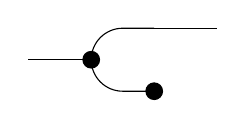
\begin{tikzpicture}[x=0.8cm, y=0.4cm, baseline]
   \draw[rounded corners=0.4cm] (1,1) -- (0,1) -- (0,0);
   \draw[rounded corners=0.4cm] (1,-1) -- (0,-1) -- (0,0);
   \draw (1,1) -- (2,1);
   \draw (0,0) -- (-1,0);
   \draw[fill=black] (0,0) circle (3pt);
   \draw[fill=black] (1,-1) circle (3pt);
  \end{tikzpicture}
 \]
\end{dfnx*}



\begin{tcbex} \par
 An internal monoid in $(\mathbf{Set}, \times, \{\ast\})$ is a monoid. An internal comonoid in  $(\mathbf{Set}, \times, \{\ast\})$ is a comonoid.
 \par
 An internal monoid in $(\mathbf{Vect}_\Bbbk, \tensor, \Bbbk)$ is a $\Bbbk$-algebra. An internal comonoid in $(\mathbf{Vect}_\Bbbk, \tensor, \Bbbk)$ is a $\Bbbk$-coalgebra.
 \par
 An  internal monoid in $(\mathbf{Cat}, \times, \mathbf{1})$, where $\mathbf{1}$ is the category with only one object, is a monoidal category. Although we have not done so, we can also define a comonoidal category, which will exactly be the comonoid in $(\mathbf{Cat}, \times, \mathbf{1})$
\end{tcbex}

As we did for monoidal categories and $\Bbbk$-algebras we are able to define morphisms between internal monoids and comonoids.

\begin{tcbdfn}[Homomorphisms of internal monoids]
 Let $(\cat{C}, \sq, I)$ be a monoidal category. An \emph{homomorphisms of internal monoids} $\varphi \colon (M, \mu, \eta) \to (M', \mu', \eta')$ is a morphism from $M$ to $M'$ such that the following diagrams commute.
 \[
  \begin{tikzcd}
   M \sq M \arrow[d, "\mu"] \arrow[r, "\varphi"] & M' \sq M' \arrow[d, "\mu'"] \\
   M \arrow[r, "\varphi"] & M'
  \end{tikzcd}
  \hspace{3em}
  \begin{tikzcd}
   M \arrow[rr, "\varphi"] & & M'\\
   & I \arrow[ul, "\eta"] \arrow[ur, "\eta'", swap] &
  \end{tikzcd}
 \]
\end{tcbdfn}


\begin{tcbdfn}[Homomorphisms of internal comonoids]
 Let $(\cat{C}, \sq, I)$ be a monoidal category. An \emph{homomorphisms of internal comonoids} $\phi \colon (M, \delta, \varepsilon) \to (M', \delta', \varepsilon')$ is a morphism from $M$ to $M'$ such that the following diagrams commute.
 \[
  \begin{tikzcd}
   M \sq M \arrow[r, "\phi"] & M' \sq M' \\
   M \arrow[u, "\delta", swap] \arrow[r, "\phi"] & M' \arrow[u, "\delta'", swap]
  \end{tikzcd}
  \hspace{3em}
  \begin{tikzcd}
   M \arrow[rr, "\phi"] \arrow[dr, "\varepsilon", swap]& & M' \arrow[dl, "\varepsilon'"] \\
   & I &
  \end{tikzcd}
 \]
\end{tcbdfn}

It is rather easy to check how composition of two morphisms of internal monoids (resp. comonoids) is again a morphism of internal monoids (resp. comonoids). Given a monoidal category $(\cat{C}, \sq, I)$, we can define a new category $\mathbf{Mon}(\cat{C})$\index{$\mathbf{Mon}(\cat{C})$, a category of internal monoids} where objects are internal monoids in $\cat{C}$ and arrows are the homomorphisms between them.

\begin{tcblemma}\label{lem:product-of-monoids}
 Let $(\cat{C}, \sq, I, \beta)$ be a symmetric monoidal category. Then $\mathbf{Mon}(\cat{C})$ can be canonically equipped with a monoidal structure.
\end{tcblemma}

\begin{proof}
 Let us take two internal monoids $(M, \mu, \eta)$, $(M', \mu', \eta')$ and define a structure of monoidal product on $M \sq M'$.
 To do so, we define the multiplication $\mu \varsq \mu$ as $(\mu \sq \mu') \circ (\id_M \sq \beta \sq \id_{M'})$.
 \[
  \begin{tikzcd}
   (M \sq M') \sq (M \sq M') \arrow[r, "\mu \varsq \mu'"] \arrow[d, "\id_M \sq \beta \sq \id_{M'}", swap] & M \sq M' \\
   M \sq M \sq M' \sq M' \arrow[ur, "\mu \sq \mu'", swap] &
  \end{tikzcd}
 \]
 We define the unit by just taking the monoidal product $\eta \sq \eta'$ and check that $(M \sq M', \mu \varsq \mu', \eta \sq \eta')$ satisfies the internal monoid axioms.
 To do so we can rely on a graphical representation of multiplication and unit.
 \[
  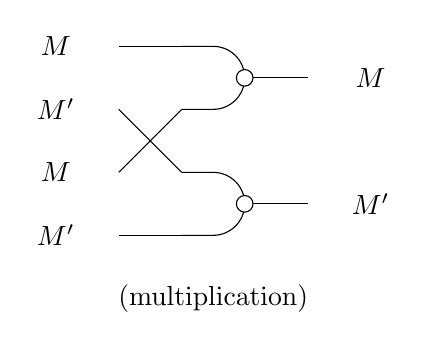
\begin{tikzpicture}[x=0.8cm, y=0.4cm, baseline]
   \draw (0,-3)--(1,-3);
   \draw (0,-1)--(1,1);
   \draw (0,1)--(1,-1);
   \draw (0,3)--(1,3);
   \draw[rounded corners=0.4cm] (1,3) -- (2,3) -- (2,2);
   \draw[rounded corners=0.4cm] (1,1) -- (2,1) -- (2,2);
   \draw[rounded corners=0.4cm] (1,-1) -- (2,-1) -- (2,-2);
   \draw[rounded corners=0.4cm] (1,-3) -- (2,-3) -- (2,-2);
   \draw (2,2)--(3,2);
   \draw (2, -2)--(3,-2);
   \draw[fill=white] (2,2) circle (3pt);
   \draw[fill=white] (2,-2) circle (3pt);
   \node (m) at (-1,3) {$M$};
   \node (m) at (-1,1) {$M'$};
   \node (m) at (-1,-1) {$M$};
   \node (m) at (-1,-3) {$M'$};
   \node (m) at (4,2) {$M$};
   \node (m) at (4,-2) {$M'$};
   \node (l) at (1.5, -5) {(multiplication)};
  \end{tikzpicture}
  \hspace{5em}
  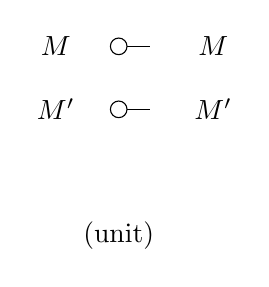
\begin{tikzpicture}[x=0.8cm, y=0.4cm, baseline]
   \draw (.5, 1)--(1,1);
   \draw (.5, -1)--(1, -1);
   \draw[fill=white] (.5, 1) circle (3pt);
   \draw[fill=white] (.5, -1) circle (3pt);
   \node (m) at (-.5,1) {$M$};
   \node (m) at (-.5,-1) {$M'$};
   \node (m) at (2,1) {$M$};
   \node (m) at (2,-1) {$M'$};
   \node (l) at (.5, -5) {(unit)};
  \end{tikzpicture}
 \]

 We hence have the associativity.
 \[
  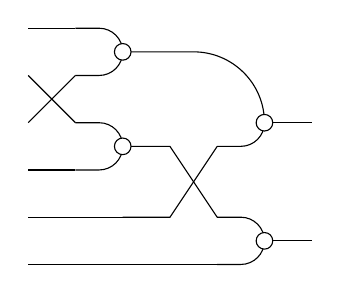
\begin{tikzpicture}[x=0.6cm, y=0.3cm, baseline]
   \draw (0, -5)--(2,-5);
   \draw (0,-3)--(2,-3);
   \draw (0,-1)--(1,-1);
   \draw (0,1)--(1,3);
   \draw (0,3)--(1,1);
   \draw (0, 5)--(1,5);
   \draw[rounded corners=0.3cm] (1,5) -- (2,5) -- (2,4);
   \draw[rounded corners=0.3cm] (1,3) -- (2,3) -- (2,4);
   \draw[rounded corners=0.3cm] (1,1) -- (2,1) -- (2,0);
   \draw[rounded corners=0.3cm] (1,-1) -- (2,-1) -- (2,0);
   \draw (2,0)--(3,0)--(4,-3);
   \draw (2,-3)--(3,-3)--(4,0);
   \draw (2,-5)--(4,-5);
   \draw[rounded corners=0.9cm] (2,4) -- (5,4) -- (5,1);
   \draw[rounded corners=0.3cm] (4,0) -- (5,0) -- (5,1);
   \draw[rounded corners=0.3cm] (4,-3) -- (5,-3) -- (5,-4);
   \draw[rounded corners=0.3cm] (4,-5) -- (5,-5) -- (5,-4);
   \draw (5,1)--(6,1);
   \draw (5,-4)--(6,-4);
   \draw[fill=white] (2,4) circle (3pt);
   \draw[fill=white] (2,0) circle (3pt);
   \draw[fill=white] (5,1) circle (3pt);
   \draw[fill=white] (5,-4) circle (3pt);
  \end{tikzpicture}
  \:\overset{\text{nat.}}{=}\:
  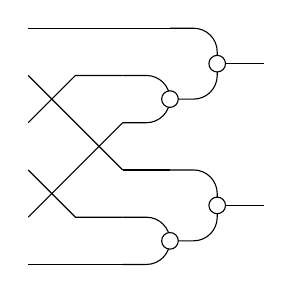
\begin{tikzpicture}[x=0.6cm, y=0.3cm, baseline]
   \draw (0, -5)--(2,-5);
   \draw (0,-3)--(1,-1)--(2,1);
   \draw (0,-1)--(1,-3)--(2,-3);
   \draw (0,1)--(1,3)--(2,3);
   \draw (0,3)--(1,1)--(2,-1);
   \draw (0,5)--(3,5);
   \draw[rounded corners=0.3cm] (2,3) -- (3,3) -- (3,2);
   \draw[rounded corners=0.3cm] (2,1) -- (3,1) -- (3,2);
   \draw[rounded corners=0.3cm] (2,-3) -- (3,-3) -- (3,-4);
   \draw[rounded corners=0.3cm] (2,-5) -- (3,-5) -- (3,-4);
   \draw (2,-1) --(3,-1);
   \draw[rounded corners=0.3cm] (3,5) -- (4,5) -- (4,3.5);
   \draw[rounded corners=0.3cm] (3,2) -- (4,2) -- (4,3.5);
   \draw[rounded corners=0.3cm] (3,-1) -- (4,-1) -- (4,-2.5);
   \draw[rounded corners=0.3cm] (3,-4) -- (4,-4) -- (4,-2.5);
   \draw (4,3.5) --(5,3.5);
   \draw (4,-2.5) --(5,-2.5);
   \draw[fill=white] (3,2) circle (3pt);
   \draw[fill=white] (3,-4) circle (3pt);
   \draw[fill=white] (4,3.5) circle (3pt);
   \draw[fill=white] (4,-2.5) circle (3pt);
  \end{tikzpicture}
  \:\overset{\text{ass.}}{=}
 \]
 \[
  \overset{\text{ass.}}{=} \:
  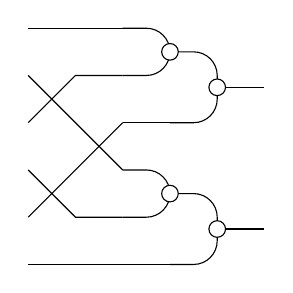
\begin{tikzpicture}[x=0.6cm, y=0.3cm, baseline]
   \draw (0, -5)--(3,-5);
   \draw (0,-3)--(1,-1)--(2,1);
   \draw (0,-1)--(1,-3)--(2,-3);
   \draw (0,1)--(1,3)--(2,3);
   \draw (0,3)--(1,1)--(2,-1);
   \draw (0,5)--(2,5);
   \draw[rounded corners=0.3cm] (2,3) -- (3,3) -- (3,4);
   \draw[rounded corners=0.3cm] (2,5) -- (3,5) -- (3,4);
   \draw[rounded corners=0.3cm] (2,-3) -- (3,-3) -- (3,-2);
   \draw[rounded corners=0.3cm] (2,-1) -- (3,-1) -- (3,-2);
   \draw (2,1) --(3,1);
   \draw[rounded corners=0.3cm] (3,-5) -- (4,-5) -- (4,-3.5);
   \draw[rounded corners=0.3cm] (3,-2) -- (4,-2) -- (4,-3.5);
   \draw[rounded corners=0.3cm] (3,1) -- (4,1) -- (4,2.5);
   \draw[rounded corners=0.3cm] (3,4) -- (4,4) -- (4,2.5);
   \draw (4,-3.5) --(5,-3.5);
   \draw (4,2.5) --(5,2.5);
   \draw[fill=white] (3,-2) circle (3pt);
   \draw[fill=white] (3,4) circle (3pt);
   \draw[fill=white] (4,-3.5) circle (3pt);
   \draw[fill=white] (4,2.5) circle (3pt);
  \end{tikzpicture}
  \:\overset{\text{nat.}}{=}\:
  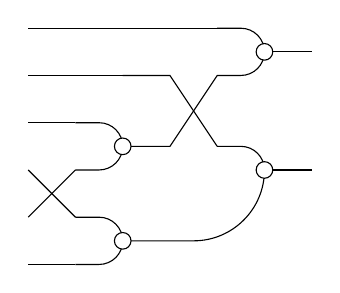
\begin{tikzpicture}[x=0.6cm, y=0.3cm, baseline]
   \draw (0, 5)--(2,5);
   \draw (0,3)--(2,3);
   \draw (0,1)--(1,1);
   \draw (0,-1)--(1,-3);
   \draw (0,-3)--(1,-1);
   \draw (0,-5)--(1,-5);
   \draw[rounded corners=0.3cm] (1,-5) -- (2,-5) -- (2,-4);
   \draw[rounded corners=0.3cm] (1,-3) -- (2,-3) -- (2,-4);
   \draw[rounded corners=0.3cm] (1,-1) -- (2,-1) -- (2,0);
   \draw[rounded corners=0.3cm] (1,1) -- (2,1) -- (2,0);
   \draw (2,0)--(3,0)--(4,3);
   \draw (2,3)--(3,3)--(4,0);
   \draw (2,5)--(4,5);
   \draw[rounded corners=0.9cm] (2,-4) -- (5,-4) -- (5,-1);
   \draw[rounded corners=0.3cm] (4,0) -- (5,0) -- (5,-1);
   \draw[rounded corners=0.3cm] (4,3) -- (5,3) -- (5,4);
   \draw[rounded corners=0.3cm] (4,5) -- (5,5) -- (5,4);
   \draw (5,-1)--(6,-1);
   \draw (5,4)--(6,4);
   \draw[fill=white] (2,-4) circle (3pt);
   \draw[fill=white] (2,0) circle (3pt);
   \draw[fill=white] (5,-1) circle (3pt);
   \draw[fill=white] (5,4) circle (3pt);
  \end{tikzpicture}
 \]
 \todo{da finire}
\end{proof}

\begin{tcbdfn}[Commutative internal monoids]
 Let $(\cat{C}, \sq, I, \beta)$ be a symmetric monoidal category. An internal monoid $(M, \mu, \eta)$ in $\cat{C}$ is \emph{commutative}\index{internal monoids!commutative internal monoids} if its multiplication is compatible with the twist map. Equivalentely we are asking for the following diagram to commute.
 \[
  \begin{tikzcd}
   M \sq M \arrow[rr, "\mu"] \arrow[dr, "\beta", swap] & & M \\
   & M \sq M \arrow[ur, "\mu", swap] &
  \end{tikzcd}
 \]
\end{tcbdfn}
The above requirement can be represented through wires as
\[
 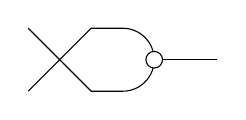
\begin{tikzpicture}[x=0.8cm, y=0.4cm, baseline]
  \draw[rounded corners=0.4cm] (-1,1) -- (0,1) -- (0,0);
  \draw[rounded corners=0.4cm] (-1,-1) -- (0,-1) -- (0,0);
  \draw (0,0) -- (1,0);
  \draw (-2,-1) -- (-1,1);
  \draw (-2,1) -- (-1,-1);
  \draw[fill=white] (0,0) circle (3pt);
 \end{tikzpicture}
 \quad=\quad
 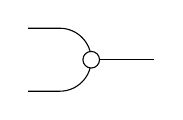
\begin{tikzpicture}[x=0.8cm, y=0.4cm, baseline]
  \draw[rounded corners=0.4cm] (-1,1) -- (0,1) -- (0,0);
  \draw[rounded corners=0.4cm] (-1,-1) -- (0,-1) -- (0,0);
  \draw (0,0) -- (1,0);
  \draw[fill=white] (0,0) circle (3pt);
 \end{tikzpicture}
\]

Similarly, we can define an analogous notion for internal comonoids.
\begin{tcbdfn}[Cocommutative internal comonoids]
 Let $(\cat{C}, \sq, I, \beta)$ be a symmetric monoidal category. An internal comonoid $(M, \delta, \varepsilon)$ in $\cat{C}$ is \emph{cocommutative}\index{internal comonoids!cocommutative internal comonoids} if its comultiplication is compatible with the twist map. Equivalentely we are asking for the following diagram to commute.
 \[
  \begin{tikzcd}
   M \arrow[rr, "\delta"] \arrow[dr, "\delta", swap] & & M \sq M \\
   & M \sq M \arrow[ur, "\beta", swap] &
  \end{tikzcd}
 \]
\end{tcbdfn}
which can be represented graphically as
\[
 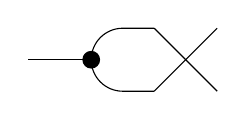
\begin{tikzpicture}[x=0.8cm, y=0.4cm, baseline]
  \draw[rounded corners=0.4cm] (1,1) -- (0,1) -- (0,0);
  \draw[rounded corners=0.4cm] (1,-1) -- (0,-1) -- (0,0);
  \draw (0,0) -- (-1,0);
  \draw (2,-1) -- (1,1);
  \draw (2,1) -- (1,-1);
  \draw[fill=black] (0,0) circle (3pt);
 \end{tikzpicture}
 \quad=\quad
 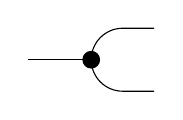
\begin{tikzpicture}[x=0.8cm, y=0.4cm, baseline]
  \draw[rounded corners=0.4cm] (1,1) -- (0,1) -- (0,0);
  \draw[rounded corners=0.4cm] (1,-1) -- (0,-1) -- (0,0);
  \draw (0,0) -- (-1,0);
  \draw[fill=black] (0,0) circle (3pt);
 \end{tikzpicture}
\]

\begin{tcblemma}\label{lem:monoid_image}
 Let $(\cat{C}, \sq, I)$, $(\cat{D}, \varsq, J)$ be two monoidal categories and let $F \colon \cat{C} \to \cat{D}$ be a (lax) monoidal functor between the two. Then, given an internal monoid $(M, \mu, \eta)$ in $\cat{C}$, its image $(F(M), F(\mu), F(\eta))$ defines an internal monoid in $\cat{D}$.
\end{tcblemma}
\begin{proof}
 The proof of this statement follows by applying Definition \ref{dfn:monoidal-functor} to the internal monoid structure.
\end{proof}

We can now construct an equivalence relation in some way analogous to our main one. This will help us generalize it later on.

\begin{tcbdfn}[The simplex category]\label{dfn:delta-cat}
 The \emph{simplex category\footnotemark} $\Delta$\index{simplex category} is the category defined by taking
 \begin{itemize}
  \item finite totally ordered sets $[n] \coloneq \{ 0, 1, 2, \dots, n-1 \}$ as objects
  \item order preserving maps as arrows
 \end{itemize}
\end{tcbdfn}
\footnotetext{This structure is sometimes referred to as the \emph{skeletal augmented simplex category}.}

We will then have $[0] = \varnothing$, $[1] = \{0\}$, $[2] = \{0, 1\}$ and so on. It is worth noticing that, in the category $\Delta$, $[0]$ is an initial object and $[1]$ is terminal object.

\begin{tcbdfn}[Ordinal sum]\label{dfn:ordinal-sum}
 The \emph{ordinal sum} is a bifunctor $+ \colon \Delta \times \Delta \to \Delta$ defined in the following way.
 \par
 \textbf{(Objects:).} Consider any two objects $[m]$, $[n]$. Their ordinal sum is defined as the object $[m+n]$ with inclusions given by:
 \begin{align*}
  [m] & \to [m+n] & [n] & \to [m+n]     \\
  i   & \mapsto i & i   & \mapsto m + i
 \end{align*}
 \par
 \textbf{(Arrows:)} Consider any two arrows $f \colon [m] \to [n]$, $f' \colon [m'] \to [n']$. Their ordinal sum is $f + f' \colon [m+m'] \to [n+n']$ assigning
 \[
  i \mapsto
  \begin{cases}
   f(i)        & \text{for } i = 0, \dots, m-1 \\
   n + f'(i-m) & \text{for } i = m, \dots, n-1
  \end{cases}
 \]
\end{tcbdfn}

Similarly to the sum we are accostumed to, the ordinal sum we just defined has $[0] = \varnothing$ as the neutral element.

Furthermore, this operation defines a monoidal structure $(\Delta, +, [0])$. We hence investigate generators and relations starting from some known \todo{add reference} properties of $\Delta$
\todo{sistemare la footnote}
\footnote{Alternatively we could completely define $\Delta$ graphically, without reliying on simplicial relations. Such approach can be found in [Kock]}.

\begin{tcblemma}
 Every arrow in $\Delta$ can be obtained as a composition of
 \begin{align*}
  \delta^n_k \colon [n] & \to [n+1] \quad \text{for $k= 0, \dots n$, called \emph{(co)face maps}} \\
  i                     & \mapsto
  \begin{cases}
   i   & \text{for } i < k    \\
   i+1 & \text{for } i \geq k
  \end{cases}
 \end{align*}
 \begin{align*}
  \sigma^n_k \colon [n+2] & \to [n+1] \quad \text{for $k= 0, \dots n$, called \emph{(co)degeneracy maps}} \\
  i                       & \mapsto
  \begin{cases}
   i   & \text{for } i \leq k \\
   i-1 & \text{for } i > k
  \end{cases}
 \end{align*}
 satisfying the so called \emph{(co)simplicial identities}.
 \begin{align}
  \delta^{n+1}_i \circ \delta^n_j & = \delta^{n+1}_{j+1} \circ \delta^{n}_i  \quad \text{for } i \leq j \label{simp1} \\
  \sigma^n_j \circ \sigma^{n+1}_i & = \sigma^n_i \circ \sigma^{n+1}_{j+1} \quad \text{for } i \leq j \label{simp2}    \\
  \sigma^n_j \circ \delta^{n+1}_i & =
  \begin{cases}
   \delta^n_i \circ \sigma^{n-1}_{j-1} & \text{for } i < j          \\
   \id                                 & \text{for } i=j, i = j + 1 \\
   \delta^n_{i-1} \circ \sigma^{n-1}_j & \text{for } i > j + 1
  \end{cases} \label{simp3}
 \end{align}
\end{tcblemma}

But what does this lemma have to do with internal monoids? The relation between the two becomes clear when we represent the two maps and their relations graphically.
We will represent each $[n]$ as a column of $n$ black dots, stacked one over the other from the bottom (element 0) to the top (element $n-1$). We begin by drawing the two maps defined in the above lemma for the case $n=3$, $k=2$.
\[
 \begin{tikzpicture}[x=1cm, y=0.4cm]
  \draw[fill=black] (0,0) circle (2pt);
  \draw[fill=black] (0,1) circle (2pt);
  \draw[fill=black] (0,2) circle (2pt);
  \draw[fill=black] (1,-.5) circle (2pt);
  \draw[fill=black] (1,.5) circle (2pt);
  \draw[fill=black] (1,1.5) circle (2pt);
  \draw[fill=black] (1,2.5) circle (2pt);
  \draw (0,0) -- (1,-.5);
  \draw (0,1) -- (1,1.5);
  \draw (0,2) -- (1,2.5);
  \node (a) at (-.5,1) {[3]};
  \node (b) at (1.5,1) {[4]};
  \node (d) at (.5,3.5) {$\delta^3_2$};
 \end{tikzpicture}
 \hspace{5em}
 \begin{tikzpicture}[x=1cm, y=0.4cm]
  \draw[fill=black] (0,0) circle (2pt);
  \draw[fill=black] (0,1) circle (2pt);
  \draw[fill=black] (0,2) circle (2pt);
  \draw[fill=black] (0,3) circle (2pt);
  \draw[fill=black] (0,4) circle (2pt);
  \draw[fill=black] (1,.5) circle (2pt);
  \draw[fill=black] (1,1.5) circle (2pt);
  \draw[fill=black] (1,2.5) circle (2pt);
  \draw[fill=black] (1,3.5) circle (2pt);
  \draw (0,0) -- (1,.5);
  \draw (0,1) -- (1,1.5);
  \draw (0,2) -- (1,1.5);
  \draw (0,3) -- (1,2.5);
  \draw (0,4) -- (1,3.5);
  \node (a) at (-.5,2) {[5]};
  \node (b) at (1.5,2) {[4]};
  \node (s) at (.5,5) {$\sigma^3_2$};
 \end{tikzpicture}
\]
Then, the relations between the two can be depicted as follows.
\begin{itemize}
 \item We compute the first relation (\ref{simp1}) for $n=2$, $i=0$, $j=1$
       \[
        \begin{tikzpicture}[x=0.8cm, y=0.4cm, baseline, yshift=-0.2cm]
         \draw[fill=black] (-1,.5) circle (2pt);
         \draw[fill=black] (0,0) circle (2pt);
         \draw[fill=black] (0,1) circle (2pt);
         \draw[fill=black] (1,-.5) circle (2pt);
         \draw[fill=black] (1,.5) circle (2pt);
         \draw[fill=black] (1,1.5) circle (2pt);
         \draw (0,0) -- (-1,.5);
         \draw (0,0) -- (1,.5);
         \draw (0,1) -- (1,1.5);
         \node (d) at (-.5,3) {$\delta_1$};
         \node (d) at (.5,3) {$\delta_0$};
        \end{tikzpicture}
        \quad=\quad
        \begin{tikzpicture}[x=0.8cm, y=0.4cm, baseline, yshift=-0.2cm]
         \draw[fill=black] (-1,.5) circle (2pt);
         \draw[fill=black] (0,0) circle (2pt);
         \draw[fill=black] (0,1) circle (2pt);
         \draw[fill=black] (1,-.5) circle (2pt);
         \draw[fill=black] (1,.5) circle (2pt);
         \draw[fill=black] (1,1.5) circle (2pt);
         \draw (0,1) -- (-1,.5);
         \draw (0,0) -- (1,-.5);
         \draw (0,1) -- (1,.5);
         \node (d) at (-.5,3) {$\delta_0$};
         \node (d) at (.5,3) {$\delta_2$};
        \end{tikzpicture}
       \]
 \item We compute the second relation (\ref{simp2}) for $n=i=j=0$.
       \[
        \begin{tikzpicture}[x=0.8cm, y=0.4cm, baseline]
         \draw[fill=black] (0,-1) circle (2pt);
         \draw[fill=black] (0,0) circle (2pt);
         \draw[fill=black] (0,1) circle (2pt);
         \draw[fill=black] (1,-.5) circle (2pt);
         \draw[fill=black] (1,.5) circle (2pt);
         \draw[fill=black] (2,0) circle (2pt);
         \draw (0,-1) -- (1,-.5);
         \draw (0,0) -- (1,-.5);
         \draw (0,1) -- (1,.5);
         \draw (2,0) -- (1,.5);
         \draw (2,0) -- (1,-.5);
         \node (d) at (.5,2.5) {$\sigma_0$};
         \node (d) at (1.5,2.5) {$\sigma_0$};
        \end{tikzpicture}
        \quad=\quad
        \begin{tikzpicture}[x=0.8cm, y=0.4cm, baseline]
         \draw[fill=black] (0,-1) circle (2pt);
         \draw[fill=black] (0,0) circle (2pt);
         \draw[fill=black] (0,1) circle (2pt);
         \draw[fill=black] (1,-.5) circle (2pt);
         \draw[fill=black] (1,.5) circle (2pt);
         \draw[fill=black] (2,0) circle (2pt);
         \draw (0,-1) -- (1,-.5);
         \draw (0,0) -- (1,.5);
         \draw (0,1) -- (1,.5);
         \draw (2,0) -- (1,.5);
         \draw (2,0) -- (1,-.5);
         \node (d) at (.5,2.5) {$\sigma_1$};
         \node (d) at (1.5,2.5) {$\sigma_0$};
        \end{tikzpicture}
       \]
 \item And we draw four different cases for the last relation
       \[
        \begin{tikzpicture}[x=0.8cm, y=0.4cm, baseline]
         \draw[fill=black] (0,-.5) circle (2pt);
         \draw[fill=black] (0,.5) circle (2pt);
         \draw[fill=black] (1,-1) circle (2pt);
         \draw[fill=black] (1,0) circle (2pt);
         \draw[fill=black] (1,1) circle (2pt);
         \draw[fill=black] (2,-.5) circle (2pt);
         \draw[fill=black] (2,.5) circle (2pt);
         \draw (0,-.5) -- (1,0);
         \draw (0,.5) -- (1,1);
         \draw (1,-1) -- (2,-.5);
         \draw (1,0) -- (2,.5);
         \draw (1,1) -- (2,.5);
         \node (d) at (.5,2.5) {$\delta_0$};
         \node (d) at (1.5,2.5) {$\sigma_1$};
        \end{tikzpicture}
        \quad=\quad
        \begin{tikzpicture}[x=0.8cm, y=0.4cm, baseline]
         \draw[fill=black] (0,-.5) circle (2pt);
         \draw[fill=black] (0,.5) circle (2pt);
         \draw[fill=black] (1,0) circle (2pt);
         \draw[fill=black] (2,-.5) circle (2pt);
         \draw[fill=black] (2,.5) circle (2pt);
         \draw (0,-.5) -- (1,0);
         \draw (0,.5) -- (1,0);
         \draw (1,0) -- (2,.5);
         \node (d) at (.5,2.5) {$\sigma_0$};
         \node (d) at (1.5,2.5) {$\delta_0$};
        \end{tikzpicture}
        \hspace{5em}
        \begin{tikzpicture}[x=0.8cm, y=0.4cm, baseline]
         \draw[fill=black] (0,-.5) circle (2pt);
         \draw[fill=black] (0,.5) circle (2pt);
         \draw[fill=black] (1,-1) circle (2pt);
         \draw[fill=black] (1,0) circle (2pt);
         \draw[fill=black] (1,1) circle (2pt);
         \draw[fill=black] (2,-.5) circle (2pt);
         \draw[fill=black] (2,.5) circle (2pt);
         \draw (0,-.5) -- (1,0);
         \draw (0,.5) -- (1,1);
         \draw (1,-1) -- (2,-.5);
         \draw (1,0) -- (2,-.5);
         \draw (1,1) -- (2,.5);
         \node (d) at (.5,2.5) {$\delta_0$};
         \node (d) at (1.5,2.5) {$\sigma_0$};
        \end{tikzpicture}
        \quad=\quad
        \begin{tikzpicture}[x=0.8cm, y=0.4cm, baseline]
         \draw[fill=black] (0,-.5) circle (2pt);
         \draw[fill=black] (0,.5) circle (2pt);
         \draw[fill=black] (1,-.5) circle (2pt);
         \draw[fill=black] (1,.5) circle (2pt);
         \draw (0,-.5) -- (1,-.5);
         \draw (0,.5) -- (1,.5);
         \node (d) at (.5,2.5) {$\id_{[2]}$};
        \end{tikzpicture}
       \]
       \[
        \begin{tikzpicture}[x=0.8cm, y=0.4cm, baseline]
         \draw[fill=black] (0,-.5) circle (2pt);
         \draw[fill=black] (0,.5) circle (2pt);
         \draw[fill=black] (1,-1) circle (2pt);
         \draw[fill=black] (1,0) circle (2pt);
         \draw[fill=black] (1,1) circle (2pt);
         \draw[fill=black] (2,-.5) circle (2pt);
         \draw[fill=black] (2,.5) circle (2pt);
         \draw (0,-.5) -- (1,-1);
         \draw (0,.5) -- (1,1);
         \draw (1,-1) -- (2,-.5);
         \draw (1,0) -- (2,-.5);
         \draw (1,1) -- (2,.5);
         \node (d) at (.5,2.5) {$\delta_1$};
         \node (d) at (1.5,2.5) {$\sigma_0$};
        \end{tikzpicture}
        \quad=\quad
        \begin{tikzpicture}[x=0.8cm, y=0.4cm, baseline]
         \draw[fill=black] (0,-.5) circle (2pt);
         \draw[fill=black] (0,.5) circle (2pt);
         \draw[fill=black] (1,-.5) circle (2pt);
         \draw[fill=black] (1,.5) circle (2pt);
         \draw (0,-.5) -- (1,-.5);
         \draw (0,.5) -- (1,.5);
         \node (d) at (.5,2.5) {$\id_{[2]}$};
        \end{tikzpicture}
        \hspace{5em}
        \begin{tikzpicture}[x=0.8cm, y=0.4cm, baseline]
         \draw[fill=black] (0,-.5) circle (2pt);
         \draw[fill=black] (0,.5) circle (2pt);
         \draw[fill=black] (1,-1) circle (2pt);
         \draw[fill=black] (1,0) circle (2pt);
         \draw[fill=black] (1,1) circle (2pt);
         \draw[fill=black] (2,-.5) circle (2pt);
         \draw[fill=black] (2,.5) circle (2pt);
         \draw (0,-.5) -- (1,-1);
         \draw (0,.5) -- (1,0);
         \draw (1,-1) -- (2,-.5);
         \draw (1,0) -- (2,-.5);
         \draw (1,1) -- (2,.5);
         \node (d) at (.5,2.5) {$\delta_2$};
         \node (d) at (1.5,2.5) {$\sigma_0$};
        \end{tikzpicture}
        \quad=\quad
        \begin{tikzpicture}[x=0.8cm, y=0.4cm, baseline]
         \draw[fill=black] (0,-.5) circle (2pt);
         \draw[fill=black] (0,.5) circle (2pt);
         \draw[fill=black] (1,0) circle (2pt);
         \draw[fill=black] (2,-.5) circle (2pt);
         \draw[fill=black] (2,.5) circle (2pt);
         \draw (0,-.5) -- (1,0);
         \draw (0,.5) -- (1,0);
         \draw (1,0) -- (2,-.5);
         \node (d) at (.5,2.5) {$\sigma_0$};
         \node (d) at (1.5,2.5) {$\delta_1$};
        \end{tikzpicture}
       \]
\end{itemize}

Since $[1]$ is a terminal object in $\Delta$ we have a unique arrow
\[ \mu^{(n)} \colon [n] \to [1] \hspace{2em} \text{for every $[n] \in \obj{\Delta}$}\]
These arrows can be drawn as
\[
 \mu^{(0)} = \:
 \begin{tikzpicture}[x=0.8cm, y=0.4cm, baseline]
  \draw[fill=black] (1,0) circle (2pt);
  \draw (.5,0) -- (1,0);
  %    \node (d) at (0,0) {$\varnothing$};
 \end{tikzpicture}
 \:\text{,}
 \quad
 \mu^{(1)} = \:
 \begin{tikzpicture}[x=0.8cm, y=0.4cm, baseline]
  \draw[fill=black] (0,0) circle (2pt);
  \draw[fill=black] (1,0) circle (2pt);
  \draw (0,0) -- (1,0);
 \end{tikzpicture}
 \:\text{,}
 \quad
 \mu^{(2)} = \:
 \begin{tikzpicture}[x=0.8cm, y=0.4cm, baseline]
  \draw[fill=black] (0,-.5) circle (2pt);
  \draw[fill=black] (0,.5) circle (2pt);
  \draw[fill=black] (1,0) circle (2pt);
  \draw (0,-.5) -- (1,0);
  \draw (0,.5) -- (1,0);
 \end{tikzpicture}
 \:\text{,}
 \quad
 \mu^{(3)} = \:
 \begin{tikzpicture}[x=0.8cm, y=0.4cm, baseline]
  \draw[fill=black] (0,-1) circle (2pt);
  \draw[fill=black] (0,0) circle (2pt);
  \draw[fill=black] (0,1) circle (2pt);
  \draw[fill=black] (1,0) circle (2pt);
  \draw (0,-1) -- (1,0);
  \draw (0,0) -- (1,0);
  \draw (0,1) -- (1,0);
 \end{tikzpicture}
 \:\text{, \dots}
\]

We can hence rewrite the above lemma in the following way:
\begin{tcblemma}\label{lem:graphical-delta}
 The monoidal category $(\Delta, +, [0])$ is completely generated\index{simplex category!generating set} in the sense of Definition \ref{dfn:generators} by the morphisms
 % \[ 
 % \mu^{(0)} \colon [0] \to [1] 
 % \quad \text{and} \quad 
 % \mu^{(2)} \colon [2] \to [1] 
 % \]
 \[
  \begin{tikzpicture}[x=0.8cm, y=0.4cm, baseline]
   \draw[fill=black] (0,.5) circle (2pt);
   \draw[fill=black] (0,-.5) circle (2pt);
   \draw[fill=black] (1,0) circle (2pt);
   \draw (0,.5) -- (1,0);
   \draw (0,-.5) -- (1,0);
   \node (mu) at (0.5, -2) {$\mu^{(2)} \colon [2] \to [1]$};
  \end{tikzpicture}
  \quad \text{and} \quad
  \begin{tikzpicture}[x=0.8cm, y=0.4cm, baseline]
   \draw[fill=black] (1,0) circle (2pt);
   \draw(1,0) -- (.5,0);
   \node (mu) at (0.5, -2) {$\mu^{(0)} \colon [0] \to [1]$};
  \end{tikzpicture}
 \]
 satisfying the following relations:
 \begin{itemize}
  \item identity relations
        \[
         \begin{tikzpicture}[x=0.8cm, y=0.4cm, baseline]
          \draw[fill=black] (0,-.5) circle (2pt);
          \draw[fill=black] (0,.5) circle (2pt);
          \draw[fill=black] (1,-.5) circle (2pt);
          \draw[fill=black] (1,.5) circle (2pt);
          \draw[fill=black] (2,0) circle (2pt);
          \draw (0,-.5) -- (1,-.5);
          \draw (0,.5) -- (1,.5);
          \draw (1,-.5) -- (2,0);
          \draw (1,.5) -- (2,0);
         \end{tikzpicture}
         \: = \:
         \begin{tikzpicture}[x=0.8cm, y=0.4cm, baseline]
          \draw[fill=black] (0,-.5) circle (2pt);
          \draw[fill=black] (0,.5) circle (2pt);
          \draw[fill=black] (1,0) circle (2pt);
          \draw[fill=black] (2,0) circle (2pt);
          \draw (0,-.5) -- (1,0);
          \draw (0,.5) -- (1,0);
          \draw (2,0) -- (1,0);
         \end{tikzpicture}
         \: = \:
         \begin{tikzpicture}[x=0.8cm, y=0.4cm, baseline]
          \draw[fill=black] (0,-.5) circle (2pt);
          \draw[fill=black] (0,.5) circle (2pt);
          \draw[fill=black] (1,0) circle (2pt);
          \draw (0,-.5) -- (1,0);
          \draw (0,.5) -- (1,0);
         \end{tikzpicture}
         \hspace{3em}
         \begin{tikzpicture}
          [x=0.8cm, y=0.4cm, baseline]
          \draw[fill=black] (0,0) circle (2pt);
          \draw[fill=black] (1,0) circle (2pt);
          \draw (-.5,0) -- (1,0);
         \end{tikzpicture}
         \: = \:
         \begin{tikzpicture}
          [x=0.8cm, y=0.4cm, baseline]
          \draw[fill=black] (0,0) circle (2pt);
          \draw[fill=black] (1,0) circle (2pt);
          \draw (0,0) -- (1,0);
         \end{tikzpicture}
        \]
  \item unitality
        \[
         \begin{tikzpicture}[x=0.8cm, y=0.4cm, baseline]
          \draw[fill=black] (0,.5) circle (2pt);
          \draw[fill=black] (1,-.5) circle (2pt);
          \draw[fill=black] (1,.5) circle (2pt);
          \draw[fill=black] (2,0) circle (2pt);
          \draw (.5,-.5) -- (1,-.5);
          \draw (0,.5) -- (1,.5);
          \draw (1,-.5) -- (2,0);
          \draw (1,.5) -- (2,0);
         \end{tikzpicture}
         \: = \:
         \begin{tikzpicture}[x=0.8cm, y=0.4cm, baseline]
          \draw[fill=black] (0,-.5) circle (2pt);
          \draw[fill=black] (1,-.5) circle (2pt);
          \draw[fill=black] (1,.5) circle (2pt);
          \draw[fill=black] (2,0) circle (2pt);
          \draw (0,-.5) -- (1,-.5);
          \draw (.5,.5) -- (1,.5);
          \draw (1,-.5) -- (2,0);
          \draw (1,.5) -- (2,0);
         \end{tikzpicture}
         \: = \:
         \begin{tikzpicture}
          [x=0.8cm, y=0.4cm, baseline]
          \draw[fill=black] (0,0) circle (2pt);
          \draw[fill=black] (1,0) circle (2pt);
          \draw (0,0) -- (1,0);
         \end{tikzpicture}
        \]
  \item associativity \[
         \begin{tikzpicture}[x=0.8cm, y=0.4cm, baseline]
          \draw[fill=black] (0,-1) circle (2pt);
          \draw[fill=black] (0,0) circle (2pt);
          \draw[fill=black] (0,1) circle (2pt);
          \draw[fill=black] (1,-.5) circle (2pt);
          \draw[fill=black] (1,.5) circle (2pt);
          \draw[fill=black] (2,0) circle (2pt);
          \draw (0,-1) -- (1,-.5);
          \draw (0,0) -- (1,-.5);
          \draw (0,1) -- (1,.5);
          \draw (2,0) -- (1,.5);
          \draw (2,0) -- (1,-.5);
         \end{tikzpicture}
         \quad=\quad
         \begin{tikzpicture}[x=0.8cm, y=0.4cm, baseline]
          \draw[fill=black] (0,-1) circle (2pt);
          \draw[fill=black] (0,0) circle (2pt);
          \draw[fill=black] (0,1) circle (2pt);
          \draw[fill=black] (1,-.5) circle (2pt);
          \draw[fill=black] (1,.5) circle (2pt);
          \draw[fill=black] (2,0) circle (2pt);
          \draw (0,-1) -- (1,-.5);
          \draw (0,0) -- (1,.5);
          \draw (0,1) -- (1,.5);
          \draw (2,0) -- (1,.5);
          \draw (2,0) -- (1,-.5);
         \end{tikzpicture}
        \]
 \end{itemize}
\end{tcblemma}

These axioms carry a striking resemblance to the ones we drew above, when describing the notion of internal monoid. We can hence state that $([1], \mu^{(2)}, \mu^{(0)})$ is a monoid in the monoidal category $(\Delta, +, [0])$. Since this monoid completely generates the whole category we have the following lemma.
\begin{tcblemma}
 The simplex category $(\Delta, +, [0])$ is the free monoidal category on a single monoid, namely $([1], \mu^{(2)}, \mu^{(0)})$.
\end{tcblemma}
More is actually true.

\begin{tcbthm}\label{thm:delta-eq}
 Given a monoidal category $(\cat{C}, \sq, I)$ there is a canonical equivalence of categories
 \[
  \mathbf{MonCat}(\Delta, \cat{C}) \iso \mathbf{Mon}(\cat{C})
 \]
\end{tcbthm}

\begin{proof}
 To prove the statement holds we need to define the functors in both directions and check they really are inverses to each other.

 We start from left to right, defining a functor $\phi \colon\mathbf{MonCat}(\Delta, \cat{C}) \to \mathbf{Mon}(\cat{C})$.
 Given a monoidal functor $F \colon \Delta \to \cat{C}$, we can just evaluate it on the monoid $([1], \mu^{(2)}, \mu^{(0)})$. By Lemma $\ref{lem:monoid_image}$, we obtain an internal monoid $(F([1]), F(\mu^{(2)}), F(\mu^{(0)}))$ in $\cat{C}$. Now, let $u \colon F \Rightarrow G$ be a monoidal natural transformation and consider its component $u_{[1]} \colon F([1]) \to G([1])$. The naturality of $u$ with respect to the generating maps of $\Delta$, ensures the compatibility of $u_{[1]}$ with the monoid structure. This means that $u_{[1]}$ defines a morphism of internal monoids in $\cat{C}$.

 Conversly, given a monoid $(M, \mu, \eta)$ in $\cat{C}$, we define a monoidal functor $F_M \colon \Delta \to \cat{C}$ as follows
 \begin{align*}
  F_M \colon \Delta              & \to \cat{C}                        \\
  [1]                            & \mapsto M                          \\
  (\mu^{(2)} \colon [2] \to [1]) & \mapsto (\mu \colon M \sq M \to M) \\
  (\mu^{(0)} \colon [0] \to [1]) & \mapsto (\eta \colon I \to M)
 \end{align*}
 This association properly defines a functor because the relations of internal monoid are the same holding between $\mu^{(0)}$ and $\mu^{(2)}$.
 Given an homomorphism of monoids $\varphi \colon (M, \mu, \eta) \to (M', \mu', \eta')$, we then define a natural transformation $u \colon F_M \Rightarrow F_{M'}$ as:
 \[
  u_1 = \phi \colon F_M([1]) = M \to F_{M'}([1]) = M'
 \]
 \[
  u_n = \underbrace{u_1 \sq \dots \sq u_1}_\text{$n$ times}
 \]
 This determines a monoidal natural transformation between the two functors, therefore a well defined functor $\psi \colon \mathbf{Mon}(\cat{C}) \to \moncat(\Delta, \cat{C})$.

 Finally we want to check the two functors just defined are inverses to each other. We hence take a natural transformation $u \colon F \Rightarrow G$ in $\mathbf{MonCat}(\Delta, \cat{C})$ and compute its image through $\phi$. We obtain the homomorphism of monoids
 \[
  F(u) = u_1 \colon (F([1]), F(\mu^{(2)}), F(\mu^{(0)})) \to (G([1]), G(\mu^{(2)}), G(\mu^{(0)}))
 \]
 to which we apply the functor $\psi$. Its image will be a natural transformation between the functors $F_{F([1])}$ and $F_{G([1])}$. Let us notice how, by definition of $\psi$, the functor $F_{F([1])}$ sends $[1]$ to $F([1])$, $\mu^{(2)}$ to $F(\mu^{(2)})$ and $\mu^{(0)}$ to $F(\mu^{(0)})$. We then have $F_{F([1])} = F$ and, by the same argument, $F_{G([1])} = G$. The natural transformation between the two is then equal to the one defined monoidally on $u_1$, hence $u \colon F \Rightarrow G$ itself.
\end{proof}

\begin{remark}
 The equivalence also holds when considering internal comonoids. In such case we'll need to consider the category $\Delta^{op}$, generated by
 \[
  \begin{tikzpicture}[x=0.8cm, y=0.4cm, baseline]
   \draw[fill=black] (0,.5) circle (2pt);
   \draw[fill=black] (0,-.5) circle (2pt);
   \draw[fill=black] (-1,0) circle (2pt);
   \draw (0,.5) -- (-1,0);
   \draw (0,-.5) -- (-1,0);
   \node (mu) at (-0.5, -2) {$\mu^{(2)} \colon [2] \to [1]$};
  \end{tikzpicture}
  \quad \text{and} \quad
  \begin{tikzpicture}[x=0.8cm, y=0.4cm, baseline]
   \draw[fill=black] (-1,0) circle (2pt);
   \draw(-1,0) -- (-.5,0);
   \node (mu) at (-.5, -2) {$\mu^{(0)} \colon [0] \to [1]$};
  \end{tikzpicture}
 \]
 satisfying the relations specular to the ones in \ref{lem:graphical-delta}. We then have the canonical equivalence of categories
 \[
  \mathbf{MonCat}(\Delta^{op}, \cat{C}) \iso \mathbf{Comon}(\cat{C})
 \]
\end{remark}

We still have not highlighted the connection between these general results and the equivalence we stated in \ref{thm:equiv}. To do so we just need to choose the right monoidal category. Indeed by taking $(\cat{C}, \sq, I)$ equal to $(\mathbf{Vect}_\Bbbk, \tensor, \Bbbk)$ we obtain
\[
 \moncat(\Delta, \mathbf{Vect}_\Bbbk) \iso \mathbf{Mon}(\mathbf{Vect}_\Bbbk) = \mathbf{Alg}_\Bbbk
\]
where algebras finally appear. \index{$\mathbf{Alg}_\Bbbk$, the category of $\Bbbk$-algebras}
% Define $\Phi$.
% We have an equivalence of categories 
% \[
% \mathbf{SymMonCat}(\Phi, \cat{C}) \iso \mathbf{cMon}(\cat{C})
% \]
% and
% \[
% \mathbf{SymMonCat}(\Phi^{op}, \cat{C}) \iso \mathbf{cComon}(\cat{C})
% \]
In this case we are still considering \emph{all} algebras. To restrict to the category $\mathbf{cFAlg}_\Bbbk$ we need to define some more internal structures.

\begin{tcbdfn}[Internal Frobenius objects]
 Let $(\cat{C}, \sq, I)$ be a monoidal category. An \emph{internal Frobenius object}\index{internal Frobenius object} in $\cat{C}$ is an object $M$ equipped with four morphisms
 \[
  \mu \colon M \sq M \to M \quad\text{(multiplication)}
  \hspace{3em}
  \eta \colon I \to M \quad\text{(unit)}
 \]
 \[
  \delta \colon M \to M \sq M \quad\text{(comultiplication)}
  \hspace{3em}
  \varepsilon \colon M \to I \quad\text{(counit)}
 \]
 such that the following diagrams commute
 \[
  \begin{tikzcd}[column sep=normal]
   & M \sq M \arrow[rd, "\mu"] & & M \sq M \arrow[ld, "\mu", swap]& \\
   I \sq M \arrow[ru, "\eta \sq \id_M"] \arrow[rr, "=", swap]& & M & & M \sq I \arrow[lu, "\id_M \sq \eta", swap] \arrow[ll, "="]
  \end{tikzcd}
 \]
 \[
  \begin{tikzcd}[column sep=normal]
   & M \sq M \arrow[dl, "\varepsilon \sq \id_M", swap] & & M \sq M \arrow[dr, "\id_M \sq \varepsilon"]& \\
   I \sq M & & M \arrow[ul, "\delta", swap] \arrow[ur, "\delta"] \arrow[ll, "="] \arrow[rr, "=", swap] & & M \sq I
  \end{tikzcd}
 \]
 \[
  \begin{tikzcd}
   & M \sq M \sq M \arrow[dr, "\mu \sq \id_M"] & \\
   M \sq M \arrow[r, "\mu"] \arrow[ur, "\id_M \sq \delta"] \arrow[dr, "\delta \sq \id_M", swap] & M \arrow[r, "\delta"] & M \sq M \\
   & M \sq M \sq M \arrow[ur, "\id_M \sq \mu", swap] &
  \end{tikzcd}
 \]
\end{tcbdfn}

As we did for monoids and comonoids we can give a graphical representation of these objects.
\begin{dfnx*}[Internal Frobenius objects]
 Let $(\cat{C}, \sq, I)$ be a monoidal category. An \emph{internal Frobenius object}\index{internal Frobenius object!in terms of wires} in $\cat{C}$ is an object $M$ equipped with four morphisms
 \[
  \begin{tikzpicture}[x=0.8cm, y=0.4cm, baseline]
   \draw[rounded corners=0.4cm] (-1,1) -- (0,1) -- (0,0);
   \draw[rounded corners=0.4cm] (-1,-1) -- (0,-1) -- (0,0);
   \draw (0,0) -- (1,0);
   \draw[fill=white] (0,0) circle (3pt);
   \node (mu) at (0,-3) {$\mu \colon M \sq M \to M$};
  \end{tikzpicture}
  \hspace{3em}
  \begin{tikzpicture}[x=0.8cm, y=0.4cm, baseline]
   \draw (0,0)--(1,0);
   \draw[fill=white] (0,0) circle (3pt);
   \node (eta) at (0,-3) {$\eta \colon I \to M$};
  \end{tikzpicture}
 \]
 \[
  \begin{tikzpicture}[x=0.8cm, y=0.4cm, baseline]
   \draw[rounded corners=0.4cm] (1,1) -- (0,1) -- (0,0);
   \draw[rounded corners=0.4cm] (1,-1) -- (0,-1) -- (0,0);
   \draw (0,0) -- (-1,0);
   \draw[fill=black] (0,0) circle (3pt);
   \node (delta) at (0,-3) {$\delta \colon M \to M \sq M$};
  \end{tikzpicture}
  \hspace{3em}
  \begin{tikzpicture}[x=0.8cm, y=0.4cm, baseline]
   \draw (0,0)--(-1,0);
   \draw[fill=black] (0,0) circle (3pt);
   \node (epsilon) at (0,-3) {$\epsilon \colon M \to I$};
  \end{tikzpicture}
 \]
 such that the following relations hold
 \[
  \begin{tikzpicture}[x=0.8cm, y=0.4cm, baseline]
   \draw[rounded corners=0.4cm] (-1,1) -- (0,1) -- (0,0);
   \draw[rounded corners=0.4cm] (-1,-1) -- (0,-1) -- (0,0);
   \draw (-1,-1) -- (-2,-1);
   \draw (0,0) -- (1,0);
   \draw[fill=white] (0,0) circle (3pt);
   \draw[fill=white] (-1,1) circle (3pt);
  \end{tikzpicture}
  \quad=\quad
  \begin{tikzpicture}[x=0.8cm, y=0.4cm, baseline]
   \draw (0,0) -- (1,0);
  \end{tikzpicture}
  \quad=\quad
  \begin{tikzpicture}[x=0.8cm, y=0.4cm, baseline]
   \draw[rounded corners=0.4cm] (-1,1) -- (0,1) -- (0,0);
   \draw[rounded corners=0.4cm] (-1,-1) -- (0,-1) -- (0,0);
   \draw (-1,1) -- (-2,1);
   \draw (0,0) -- (1,0);
   \draw[fill=white] (0,0) circle (3pt);
   \draw[fill=white] (-1,-1) circle (3pt);
  \end{tikzpicture}
 \]
 \[
  \begin{tikzpicture}[x=0.8cm, y=0.4cm, baseline]
   \draw[rounded corners=0.4cm] (1,1) -- (0,1) -- (0,0);
   \draw[rounded corners=0.4cm] (1,-1) -- (0,-1) -- (0,0);
   \draw (1,-1) -- (2,-1);
   \draw (0,0) -- (-1,0);
   \draw[fill=black] (0,0) circle (3pt);
   \draw[fill=black] (1,1) circle (3pt);
  \end{tikzpicture}
  \quad=\quad
  \begin{tikzpicture}[x=0.8cm, y=0.4cm, baseline]
   \draw (0,0) -- (1,0);
  \end{tikzpicture}
  \quad=\quad
  \begin{tikzpicture}[x=0.8cm, y=0.4cm, baseline]
   \draw[rounded corners=0.4cm] (1,1) -- (0,1) -- (0,0);
   \draw[rounded corners=0.4cm] (1,-1) -- (0,-1) -- (0,0);
   \draw (1,1) -- (2,1);
   \draw (0,0) -- (-1,0);
   \draw[fill=black] (0,0) circle (3pt);
   \draw[fill=black] (1,-1) circle (3pt);
  \end{tikzpicture}
 \]
 \[
  \begin{tikzpicture}[x=0.8cm, y=0.4cm, baseline,yshift=-0.25cm]
   \draw[rounded corners=0.4cm] (0,2) -- (0,1) -- (.5,1);
   \draw[rounded corners=0.4cm] (0,2) -- (0,3) -- (2,3);
   \draw[rounded corners=0.4cm] (1,0) -- (1,1) -- (.5,1);
   \draw[rounded corners=0.4cm] (1,0) -- (1,-1) -- (-1,-1);
   \draw (2,0)--(1,0);
   \draw (0,2)--(-1,2);
   \draw[fill=black] (0,2) circle (3pt);
   \draw[fill=white] (1,0) circle (3pt);
  \end{tikzpicture}
  \quad=\quad
  \begin{tikzpicture}[x=0.8cm, y=0.4cm, baseline]
   \draw[rounded corners=0.4cm] (-1,-1) -- (0,-1) -- (0,0);
   \draw[rounded corners=0.4cm] (-1,1) -- (0,1) -- (0,0);
   \draw (0,0) -- (1,0);
   \draw[fill=white] (0,0) circle (3pt);
   \draw[fill=black] (1,0) circle (3pt);
   \draw[rounded corners=0.4cm] (1,0) -- (1,1) -- (2,1);
   \draw[rounded corners=0.4cm] (1,0) -- (1,-1) -- (2,-1);
  \end{tikzpicture}
  \quad=\quad
  \begin{tikzpicture}[x=0.8cm, y=0.4cm, baseline,yshift=-0.25cm]
   \draw[rounded corners=0.4cm] (0,2) -- (0,1) -- (-.5,1);
   \draw[rounded corners=0.4cm] (0,2) -- (0,3) -- (-2,3);
   \draw[rounded corners=0.4cm] (-1,0) -- (-1,1) -- (-.5,1);
   \draw[rounded corners=0.4cm] (-1,0) -- (-1,-1) -- (1,-1);
   \draw (-2,0)--(-1,0);
   \draw (0,2)--(1,2);
   \draw[fill=white] (0,2) circle (3pt);
   \draw[fill=black] (-1,0) circle (3pt);
  \end{tikzpicture}
 \]
\end{dfnx*}



\begin{tcblemma}
 An internal Frobenius object $M$ is both an internal monoid and an internal comonoid.
\end{tcblemma}
\begin{proof}
 Let $(M, \mu, \eta, \delta, \varepsilon)$ be a Frobenius object. By proving $\mu$ and $\delta$ are associatives, we obtain an internal monoid $(M, \mu, \eta)$ and an internal comonoid $(M, \delta, \varepsilon)$. The proof of this fact is equivalent to the graphical proof of the equivalence of Frobenius algebras we gave in the previous chapter (see Proposition \ref{prp:Frobenius-equivalence}).
\end{proof}

Following this lemma, we define \emph{homomorphisms of internal Frobenius objects} to be morphisms $\varphi \colon (M, \mu, \eta, \delta, \varepsilon) \to (M', \mu', \eta', \delta', \varepsilon')$ that are homomorphisms of both the underlying monoid structure and the comonoid one. In this way, given any monoidal category $(\cat{C}, \sq, I)$, we obtain a category $\mathbf{Frob}(\cat{C})$\index{$\mathbf{Frob}(\cat{C})$, a category of internal Frobenius objects} whose objects are internal Frobenius objects in $\cat{C}$ and arrows are the homomorphisms between them.

\begin{tcblemma}\label{lem:product-of-frobenius}
 Let $(\cat{C}, \sq, I, \beta)$ be a symmetric monoidal category. Then $\mathbf{Frob}(\cat{C})$ can be canonically equipped with a monoidal structure.
\end{tcblemma}

\begin{proof}
 Let us take two internal Frobenius object $(M, \mu, \eta, \delta, \varepsilon)$, $(M', \mu', \eta', \delta', \varepsilon')$ and prove the multiplication defined in \ref{lem:product-of-monoids} together with the analogous comultiplication define an internal Frobenius object $M \sq M'$. What we need to do is proving the Frobenius relation holds.
 \[
  \begin{tikzpicture}[x=0.6cm, y=0.3cm, baseline]
   \draw (0,-5) -- (4,-5);
   \draw (0,-3) -- (3,-3);
   \draw (0,0) -- (1,0);
   \draw (0,4) -- (1,4);
   \draw (2,-1) -- (3,-1);
   \draw (5,-4) -- (6,-4);
   \draw (5,0) -- (6,0);
   \draw (3,3) -- (6,3);
   \draw (2,5) -- (6,5);
   \draw (3,1) -- (4,1);
   \draw (3,-3) -- (4,-1);
   \draw (3,-1) -- (4,-3);
   \draw (2,1) -- (3,3);
   \draw (2,3) -- (3,1);
   \draw[rounded corners=0.3cm] (1,0) -- (1,-1) -- (2,-1);
   \draw[rounded corners=0.3cm] (1,0) -- (1,1) -- (2,1);
   \draw[rounded corners=0.3cm] (1,4) -- (1,3) -- (2,3);
   \draw[rounded corners=0.3cm] (1,4) -- (1,5) -- (2,5);
   \draw[rounded corners=0.3cm] (4,-5) -- (5,-5) -- (5,-4);
   \draw[rounded corners=0.3cm] (4,-3) -- (5,-3) -- (5,-4);
   \draw[rounded corners=0.3cm] (4,1) -- (5,1) -- (5,0);
   \draw[rounded corners=0.3cm] (4,-1) -- (5,-1) -- (5,0);
   \draw[fill=black] (1,0) circle (3pt);
   \draw[fill=black] (1,4) circle (3pt);
   \draw[fill=white] (5,-4) circle (3pt);
   \draw[fill=white] (5,0) circle (3pt);
  \end{tikzpicture}
  \: = \:
  \begin{tikzpicture}[x=0.6cm, y=0.3cm, baseline]
   \draw (0,3) -- (1,3);
   \draw (0,-3) -- (1,-3);
   \draw (0,-1) -- (1,1);
   \draw (0,1) -- (1,-1);
   \draw (5,3) -- (4,3);
   \draw (5,-3) -- (4,-3);
   \draw (4,1) -- (5,-1);
   \draw (4,-1) -- (5,1);
   \draw (2,2) -- (3,2);
   \draw (2,-2) -- (3,-2);
   \draw[rounded corners=0.3cm] (1,3) -- (2,3) -- (2,2);
   \draw[rounded corners=0.3cm] (1,1) -- (2,1) -- (2,2);
   \draw[rounded corners=0.3cm] (4,3) -- (3,3) -- (3,2);
   \draw[rounded corners=0.3cm] (4,1) -- (3,1) -- (3,2);
   \draw[rounded corners=0.3cm] (1,-3) -- (2,-3) -- (2,-2);
   \draw[rounded corners=0.3cm] (1,-1) -- (2,-1) -- (2,-2);
   \draw[rounded corners=0.3cm] (4,-3) -- (3,-3) -- (3,-2);
   \draw[rounded corners=0.3cm] (4,-1) -- (3,-1) -- (3,-2);
   \draw[fill=white] (2,2) circle (3pt);
   \draw[fill=black] (3,2) circle (3pt);
   \draw[fill=white] (2,-2) circle (3pt);
   \draw[fill=black] (3,-2) circle (3pt);
  \end{tikzpicture}
  \: = \:
  \begin{tikzpicture}[x=0.6cm, y=0.3cm, baseline]
   \draw (0,5) -- (4,5);
   \draw (0,3) -- (3,3);
   \draw (0,0) -- (1,0);
   \draw (0,-4) -- (1,-4);
   \draw (2,1) -- (3,1);
   \draw (5,4) -- (6,4);
   \draw (5,0) -- (6,0);
   \draw (3,-3) -- (6,-3);
   \draw (2,-5) -- (6,-5);
   \draw (3,-1) -- (4,-1);
   \draw (3,3) -- (4,1);
   \draw (3,1) -- (4,3);
   \draw (2,-1) -- (3,-3);
   \draw (2,-3) -- (3,-1);
   \draw[rounded corners=0.3cm] (1,0) -- (1,1) -- (2,1);
   \draw[rounded corners=0.3cm] (1,0) -- (1,-1) -- (2,-1);
   \draw[rounded corners=0.3cm] (1,-4) -- (1,-3) -- (2,-3);
   \draw[rounded corners=0.3cm] (1,-4) -- (1,-5) -- (2,-5);
   \draw[rounded corners=0.3cm] (4,5) -- (5,5) -- (5,4);
   \draw[rounded corners=0.3cm] (4,3) -- (5,3) -- (5,4);
   \draw[rounded corners=0.3cm] (4,1) -- (5,1) -- (5,0);
   \draw[rounded corners=0.3cm] (4,-1) -- (5,-1) -- (5,0);
   \draw[fill=black] (1,0) circle (3pt);
   \draw[fill=black] (1,-4) circle (3pt);
   \draw[fill=white] (5,4) circle (3pt);
   \draw[fill=white] (5,0) circle (3pt);
  \end{tikzpicture}
 \]
 We prove the left-side of the equivalence, starting from the configuration in the middle. By applying the Frobenius relation we have
 \[
  \begin{tikzpicture}[x=0.6cm, y=0.3cm, baseline]
   \draw (3,-4) -- (1,-4);
   \draw (3, 5) -- (0,5);
   \draw (3, 2) -- (2,-1);
   \draw (3, -1) -- (2,2);
   \draw (2,2) -- (1,2);
   \draw (2,-1) -- (0,-1);
   \draw (-3, 4) -- (-1,4);
   \draw (-3, -5) -- (0,-5);
   \draw (-3, -2) -- (-2,1);
   \draw (-3, 1) -- (-2,-2);
   \draw (-2,-2) -- (-1,-2);
   \draw (-2,1) -- (0,1);
   \draw[rounded corners=0.3cm] (0,5) -- (-1,5) -- (-1,4);
   \draw[rounded corners=0.3cm] (0,3) -- (-1,3) -- (-1,4);
   \draw[rounded corners=0.3cm] (0,3) -- (1,3) -- (1,2);
   \draw[rounded corners=0.3cm] (0,1) -- (1,1) -- (1,2);
   \draw[rounded corners=0.3cm] (0,-5) -- (1,-5) -- (1,-4);
   \draw[rounded corners=0.3cm] (0,-3) -- (1,-3) -- (1,-4);
   \draw[rounded corners=0.3cm] (0,-3) -- (-1,-3) -- (-1,-2);
   \draw[rounded corners=0.3cm] (0,-1) -- (-1,-1) -- (-1,-2);
   \draw[fill=black] (-1,4) circle (3pt);
   \draw[fill=white] (1,-4) circle (3pt);
   \draw[fill=white] (1,2) circle (3pt);
   \draw[fill=black] (-1,-2) circle (3pt);
  \end{tikzpicture}
 \]
 By naturality of the twist, this is equivalent to
 \[
  \begin{tikzpicture}[x=0.6cm, y=0.3cm, baseline]
   \draw (4,5)--(-1,5);
   \draw (4,3)--(2,3);
   \draw (1,3)--(-1,3);
   \draw (2,-1)--(1,-1);
   \draw (2,3)--(1,1);
   \draw (2,1)--(1,3);
   \draw (0,-1)--(1,1);
   \draw (0,1)--(1,-1);
   \draw (-2,4)--(-4,4);
   \draw (3,0)--(4,0);
   \draw (-4,-5)--(1,-5);
   \draw (-4,-3)--(-2,-3);
   \draw (-1,-3)--(1,-3);
   \draw (-2,1)--(-1,1);
   \draw (-2,-3)--(-1,-1);
   \draw (-2,-1)--(-1,-3);
   \draw (0,1)--(-1,-1);
   \draw (0,-1)--(-1,1);
   \draw (2,-4)--(4,-4);
   \draw (-3,0)--(-4,0);
   \draw[rounded corners=0.3cm] (2,1) -- (3,1) -- (3,0);
   \draw[rounded corners=0.3cm] (2,-1) -- (3,-1) -- (3,0);
   \draw[rounded corners=0.3cm] (-2,1) -- (-3,1) -- (-3,0);
   \draw[rounded corners=0.3cm] (-2,-1) -- (-3,-1) -- (-3,0);
   \draw[rounded corners=0.3cm] (-1,5) -- (-2,5) -- (-2,4);
   \draw[rounded corners=0.3cm] (-1,3) -- (-2,3) -- (-2,4);
   \draw[rounded corners=0.3cm] (1,-5) -- (2,-5) -- (2,-4);
   \draw[rounded corners=0.3cm] (1,-3) -- (2,-3) -- (2,-4);
   \draw[fill=black] (-2,4) circle (3pt);
   \draw[fill=white] (2,-4) circle (3pt);
   \draw[fill=white] (3,0) circle (3pt);
   \draw[fill=black] (-3,0) circle (3pt);
  \end{tikzpicture}
 \]
 The twists in the middle vanish and we conclude our proof.
\end{proof}

This framework allows us to define an analogue of the simplex category $\Delta$ in the case of internal Frobenius objects.
\begin{tcbdfn}[A free monoidal category on an internal Frobenius object]
 Let $(\cat{F}, \sq, 0)$ be the monoidal category whose objects are the monoidal powers of a given object $F$ and whose arrows are generated in the sense of Definition \ref{dfn:generators} by
 \[
  \begin{tikzpicture}[x=0.8cm, y=0.4cm, baseline]
   \draw[fill=black] (0,.5) circle (2pt);
   \draw[fill=black] (0,-.5) circle (2pt);
   \draw[fill=black] (1,0) circle (2pt);
   \draw (0,.5) -- (1,0);
   \draw (0,-.5) -- (1,0);
   \node (mu) at (0.5, 2) {$\mu \colon F \sq F \to F$};
  \end{tikzpicture}
  \hspace{3em}
  \begin{tikzpicture}[x=0.8cm, y=0.4cm, baseline]
   \draw[fill=black] (1,0) circle (2pt);
   \draw (0.5,0) -- (1,0);
   \node (eta) at (0.5, 2) {$\eta \colon 0 \to F$};
  \end{tikzpicture}
  \hspace{3em}
  \begin{tikzpicture}[x=0.8cm, y=0.4cm, baseline]
   \draw[fill=black] (0,.5) circle (2pt);
   \draw[fill=black] (0,-.5) circle (2pt);
   \draw[fill=black] (-1,0) circle (2pt);
   \draw (0,.5) -- (-1,0);
   \draw (0,-.5) -- (-1,0);
   \node (d) at (-0.5, 2) {$\delta \colon F \to F \sq F$};
  \end{tikzpicture}
  \hspace{3em}
  \begin{tikzpicture}[x=0.8cm, y=0.4cm, baseline]
   \draw[fill=black] (-1,0) circle (2pt);
   \draw(-1,0) -- (-.5,0);
   \node (e) at (-.5, 2) {$\varepsilon \colon F \to 0$};
  \end{tikzpicture}
 \]
 satisfying the following relations:
 \[
  \begin{tikzpicture}[x=0.8cm, y=0.4cm, baseline]
   \draw[fill=black] (0,.5) circle (2pt);
   \draw[fill=black] (1,-.5) circle (2pt);
   \draw[fill=black] (1,.5) circle (2pt);
   \draw[fill=black] (2,0) circle (2pt);
   \draw (.5,-.5) -- (1,-.5);
   \draw (0,.5) -- (1,.5);
   \draw (1,-.5) -- (2,0);
   \draw (1,.5) -- (2,0);
  \end{tikzpicture}
  \: = \:
  \begin{tikzpicture}[x=0.8cm, y=0.4cm, baseline]
   \draw[fill=black] (0,-.5) circle (2pt);
   \draw[fill=black] (1,-.5) circle (2pt);
   \draw[fill=black] (1,.5) circle (2pt);
   \draw[fill=black] (2,0) circle (2pt);
   \draw (0,-.5) -- (1,-.5);
   \draw (.5,.5) -- (1,.5);
   \draw (1,-.5) -- (2,0);
   \draw (1,.5) -- (2,0);
  \end{tikzpicture}
  \: = \:
  \begin{tikzpicture}
   [x=0.8cm, y=0.4cm, baseline]
   \draw[fill=black] (0,0) circle (2pt);
   \draw[fill=black] (1,0) circle (2pt);
   \draw (0,0) -- (1,0);
  \end{tikzpicture}
  \hspace{3em}
  \begin{tikzpicture}[x=0.8cm, y=0.4cm, baseline]
   \draw[fill=black] (0,.5) circle (2pt);
   \draw[fill=black] (-1,-.5) circle (2pt);
   \draw[fill=black] (-1,.5) circle (2pt);
   \draw[fill=black] (-2,0) circle (2pt);
   \draw (-.5,-.5) -- (-1,-.5);
   \draw (0,.5) -- (-1,.5);
   \draw (-1,-.5) -- (-2,0);
   \draw (-1,.5) -- (-2,0);
  \end{tikzpicture}
  \: = \:
  \begin{tikzpicture}[x=0.8cm, y=0.4cm, baseline]
   \draw[fill=black] (0,-.5) circle (2pt);
   \draw[fill=black] (-1,-.5) circle (2pt);
   \draw[fill=black] (-1,.5) circle (2pt);
   \draw[fill=black] (-2,0) circle (2pt);
   \draw (0,-.5) -- (-1,-.5);
   \draw (-.5,.5) -- (-1,.5);
   \draw (-1,-.5) -- (-2,0);
   \draw (-1,.5) -- (-2,0);
  \end{tikzpicture}
  \: = \:
  \begin{tikzpicture}[x=0.8cm, y=0.4cm, baseline]
   \draw[fill=black] (0,0) circle (2pt);
   \draw[fill=black] (-1,0) circle (2pt);
   \draw (0,0) -- (-1,0);
  \end{tikzpicture}
 \]
 \[
  \begin{tikzpicture}[x=0.8cm, y=0.4cm, baseline]
   \draw[fill=black] (0,0) circle (2pt);
   \draw[fill=black] (1,0.5) circle (2pt);
   \draw[fill=black] (-1,0.5) circle (2pt);
   \draw[fill=black] (1,-.5) circle (2pt);
   \draw[fill=black] (-1,-.5) circle (2pt);
   \draw[fill=black] (0,1) circle (2pt);
   \draw[fill=black] (0,-1) circle (2pt);
   \draw (1,.5)--(0,1)--(-1,.5)--(0,0)--(1,-.5)--(0,-1)--(-1,-.5);
  \end{tikzpicture}
  \: = \:
  \begin{tikzpicture}[x=0.8cm, y=0.4cm, baseline]
   \draw[fill=black] (0,0) circle (2pt);
   \draw[fill=black] (1,0.5) circle (2pt);
   \draw[fill=black] (-1,0.5) circle (2pt);
   \draw[fill=black] (1,-.5) circle (2pt);
   \draw[fill=black] (-1,-.5) circle (2pt);
   \draw (1,.5)--(0,0)--(-1,-.5);
   \draw (-1,.5)--(0,0)--(1,-.5);
  \end{tikzpicture}
  \: = \:
  \begin{tikzpicture}[x=0.8cm, y=0.4cm, baseline]
   \draw[fill=black] (0,0) circle (2pt);
   \draw[fill=black] (1,0.5) circle (2pt);
   \draw[fill=black] (-1,0.5) circle (2pt);
   \draw[fill=black] (1,-.5) circle (2pt);
   \draw[fill=black] (-1,-.5) circle (2pt);
   \draw[fill=black] (0,1) circle (2pt);
   \draw[fill=black] (0,-1) circle (2pt);
   \draw (-1,.5)--(0,1)--(1,.5)--(0,0)--(-1,-.5)--(0,-1)--(1,-.5);
  \end{tikzpicture}
 \]
\end{tcbdfn}

We this definition we are able to extend theorem \ref{thm:delta-eq} to the Frobenius case.

\begin{tcbthm}
 Given a monoidal category $(\cat{C}, \sq, I)$ there is a canonical equivalence of categories
 \[
  \mathbf{MonCat}(\cat{F}, \cat{C}) \iso \mathbf{Mon}(\cat{C})
 \]
\end{tcbthm}

Since we are interested in symmetric monoidal categories, it makes sense to understand how the Frobenius structure interacts with the given twist.

\begin{tcbdfn}[Commutative Frobenius objects]
 An internal Frobenius object $(M, \mu, \eta, \delta, \varepsilon)$ in a symmetric monoidal category $(\cat{C}, \sq, I, \beta)$ is \emph{commutative}\index{internal Frobenius object!commutative internal Frobenius object} if the twist commutes with the multiplication $\mu$.
\end{tcbdfn}
\begin{tcbdfn}[Cocommutative Frobenius objects]
 An internal Frobenius object $(M, \mu, \eta, \delta, \varepsilon)$ in a symmetric monoidal category $(\cat{C}, \sq, I, \beta)$ is \emph{cocommutative}\index{internal Frobenius object!cocommutative internal Frobenius object} if the twist cocommutes with the comultiplication $\delta$.
\end{tcbdfn}

\begin{tcblemma}
 An internal Frobenius object in a symmetric monoidal category is commutative if and only if it is cocommutative.
\end{tcblemma}

\begin{proof}
 Let $(\cat{C}, \sq, I, \beta)$ be a symmetric monoidal category. Assume $(M, \mu, \eta, \delta, \varepsilon)$ is a commutative Frobenius object in $\cat{C}$ and consider the composition $\beta \circ \delta$. Having already proved in Section \ref{subsec:equiv} the uniqueness of the comultiplication, we can prove $\beta \circ \delta = \delta$ by showing that $\beta \circ \delta$ has counit $\varepsilon$ and satisfies the Frobenius relation. The first property follows by naturality of the twist:
 \[
  \begin{tikzpicture}[x=0.6cm, y=0.3cm, baseline]
   \draw[rounded corners=0.4cm] (1,1) -- (0,1) -- (0,0);
   \draw[rounded corners=0.4cm] (1,-1) -- (0,-1) -- (0,0);
   \draw (1,-1) -- (2,1);
   \draw (1,1) -- (2,-1);
   \draw (0,0) -- (-1,0);
   \draw[fill=black] (0,0) circle (2pt);
   \draw[fill=black] (2,-1) circle (2pt);
  \end{tikzpicture}
  \quad=\quad
  \begin{tikzpicture}[x=0.6cm, y=0.3cm, baseline]
   \draw[rounded corners=0.4cm] (1,1) -- (0,1) -- (0,0);
   \draw[rounded corners=0.4cm] (1,-1) -- (0,-1) -- (0,0);
   \draw (1,-1) -- (2,-1);
   \draw (0,0) -- (-1,0);
   \draw[fill=black] (0,0) circle (2pt);
   \draw[fill=black] (1,1) circle (2pt);
  \end{tikzpicture}
  \quad=\quad
  \begin{tikzpicture}[x=0.6cm, y=0.3cm, baseline]
   \draw (0,0) -- (1,0);
  \end{tikzpicture}
  \quad=\quad
  \begin{tikzpicture}[x=0.6cm, y=0.3cm, baseline]
   \draw[rounded corners=0.4cm] (1,1) -- (0,1) -- (0,0);
   \draw[rounded corners=0.4cm] (1,-1) -- (0,-1) -- (0,0);
   \draw (1,1) -- (2,1);
   \draw (0,0) -- (-1,0);
   \draw[fill=black] (0,0) circle (2pt);
   \draw[fill=black] (1,-1) circle (2pt);
  \end{tikzpicture}
  \quad=\quad
  \begin{tikzpicture}[x=0.6cm, y=0.3cm, baseline]
   \draw[rounded corners=0.4cm] (1,1) -- (0,1) -- (0,0);
   \draw[rounded corners=0.4cm] (1,-1) -- (0,-1) -- (0,0);
   \draw (1,-1) -- (2,1);
   \draw (1,1) -- (2,-1);
   \draw (0,0) -- (-1,0);
   \draw[fill=black] (0,0) circle (2pt);
   \draw[fill=black] (2,1) circle (2pt);
  \end{tikzpicture}
 \]
 Finally we prove the Frobenius relation holds.
 \[
  \begin{tikzpicture}[x=0.8cm, y=0.4cm, baseline]
   \draw[rounded corners=0.4cm] (-1,-1) -- (0,-1) -- (0,0);
   \draw[rounded corners=0.4cm] (-1,1) -- (0,1) -- (0,0);
   \draw (0,0) -- (1,0);
   \draw[fill=white] (0,0) circle (3pt);
   \draw[fill=black] (1,0) circle (3pt);
   \draw[rounded corners=0.4cm] (1,0) -- (1,1) -- (2,1);
   \draw[rounded corners=0.4cm] (1,0) -- (1,-1) -- (2,-1);
   \draw (2,1)--(3,-1);
   \draw (2,-1)--(3,1);
  \end{tikzpicture}
  \: \overset{\text{comm.}}{=}
  \begin{tikzpicture}[x=0.8cm, y=0.4cm, baseline]
   \draw[rounded corners=0.4cm] (-1,-1) -- (0,-1) -- (0,0);
   \draw[rounded corners=0.4cm] (-1,1) -- (0,1) -- (0,0);
   \draw (0,0) -- (1,0);
   \draw[fill=white] (0,0) circle (3pt);
   \draw[fill=black] (1,0) circle (3pt);
   \draw[rounded corners=0.4cm] (1,0) -- (1,1) -- (2,1);
   \draw[rounded corners=0.4cm] (1,0) -- (1,-1) -- (2,-1);
   \draw (2,1)--(3,-1);
   \draw (2,-1)--(3,1);
   \draw (-1,-1)--(-2,1);
   \draw (-1,1)--(-2,-1);
  \end{tikzpicture}
  \: \overset{\text{F}}{=}
 \]
 \[
  \overset{\text{F}}{=} \:
  \begin{tikzpicture}[x=0.8cm, y=0.4cm, baseline]
   \draw (1,1) -- (2,1);
   \draw (0,-2) -- (2,-2);
   \draw (2,1) -- (3,-2);
   \draw (2,-2) -- (3,1);
   \draw[rounded corners=0.4cm] (0,2) -- (1,2) -- (1,1);
   \draw[rounded corners=0.4cm] (0,0) -- (1,0) -- (1,1);
   \draw (-1,-1) -- (-2,-1);
   \draw (0,2) -- (-2,2);
   \draw (-2,-1) -- (-3,2);
   \draw (-2,2) -- (-3,-1);
   \draw[rounded corners=0.4cm] (0,-2) -- (-1,-2) -- (-1,-1);
   \draw[rounded corners=0.4cm] (0,0) -- (-1,0) -- (-1,-1);
   \draw[fill=white] (1,1) circle (3pt);
   \draw[fill=black] (-1,-1) circle (3pt);
  \end{tikzpicture}
  \: \overset{\text{nat.}}{=} \:
  \begin{tikzpicture}[x=0.8cm, y=0.4cm, baseline]
   \draw (0,0) -- (1,-2);
   \draw (0,-2) -- (1,0);
   \draw (1,0) -- (2,2);
   \draw (1,2) -- (2,0);
   \draw (1,-2) -- (2,-2);
   \draw (3,-1) -- (4,-1);
   \draw (0,2) -- (1,2);
   \draw[rounded corners=0.4cm] (2,0) -- (3,0) -- (3,-1);
   \draw[rounded corners=0.4cm] (2,-2) -- (3,-2) -- (3,-1);
   \draw (0,0) -- (-1,2);
   \draw (0,2) -- (-1,0);
   \draw (-1,0) -- (-2,-2);
   \draw (-1,-2) -- (-2,0);
   \draw (-1,2) -- (-2,2);
   \draw (-3,1) -- (-4,1);
   \draw (0,-2) -- (-1,-2);
   \draw[rounded corners=0.4cm] (-2,0) -- (-3,0) -- (-3,1);
   \draw[rounded corners=0.4cm] (-2,2) -- (-3,2) -- (-3,1);
   \draw[fill=black] (-3,1) circle (3pt);
   \draw[fill=white] (3,-1) circle (3pt);
  \end{tikzpicture}
  \: \overset{\text{nat.}}{=}
 \]
 \[
  \overset{\text{nat.}}{=} \:
  \begin{tikzpicture}[x=0.8cm, y=0.4cm, baseline]
   \draw (-2,2) -- (0,2);
   \draw (0,2) -- (2,-2);
   \draw (1,2) -- (2,2);
   \draw (1,2) -- (-1,-2)-- (-2,0);
   \draw (-2,-2) -- (-1,0) -- (0,-2) -- (1,-2) -- (2,0);
   \draw (-4,1) -- (-3,1);
   \draw (4,-1) -- (3,-1);
   \draw[rounded corners=0.4cm] (-2,0) -- (-3,0) -- (-3,1);
   \draw[rounded corners=0.4cm] (-2,2) -- (-3,2) -- (-3,1);
   \draw[rounded corners=0.4cm] (2,0) -- (3,0) -- (3,-1);
   \draw[rounded corners=0.4cm] (2,-2) -- (3,-2) -- (3,-1);
   \draw[fill=black] (-3,1) circle (3pt);
   \draw[fill=white] (3,-1) circle (3pt);
  \end{tikzpicture}
  \: \overset{\text{inv.}}{=} \:
  \begin{tikzpicture}[x=0.8cm, y=0.4cm, baseline]
   \draw (-1,2) -- (0,2) -- (2,-2);
   \draw (-1,0) -- (0,0) -- (1,2);
   \draw (-2,-2) -- (1,-2) -- (2,0);
   \draw (-2,1) -- (-3,1);
   \draw (4,-1) -- (3,-1);
   \draw[rounded corners=0.4cm] (-1,0) -- (-2,0) -- (-2,1);
   \draw[rounded corners=0.4cm] (-1,2) -- (-2,2) -- (-2,1);
   \draw[rounded corners=0.4cm] (2,0) -- (3,0) -- (3,-1);
   \draw[rounded corners=0.4cm] (2,-2) -- (3,-2) -- (3,-1);
   \draw[fill=black] (-2,1) circle (3pt);
   \draw[fill=white] (3,-1) circle (3pt);
  \end{tikzpicture}
  \: =
 \]
 \[
  \overset{\text{comm.}}{=} \:
  \begin{tikzpicture}[x=0.8cm, y=0.4cm, baseline]
   \draw (-3,1) -- (-2,1);
   \draw (-1,2) -- (0,0);
   \draw (-1,0) -- (0,2);
   \draw (1,-1) -- (2,-1);
   \draw[rounded corners=0.4cm] (-1,0) -- (-2,0) -- (-2,1);
   \draw[rounded corners=0.4cm] (-1,2) -- (-2,2) -- (-2,1);
   \draw[rounded corners=0.4cm] (0,0) -- (1,0) -- (1,-1);
   \draw[rounded corners=0.4cm] (0,-2) -- (1,-2) -- (1,-1);
   \draw[fill=black] (-2,1) circle (3pt);
   \draw[fill=white] (1,-1) circle (3pt);
  \end{tikzpicture}
 \]
\end{proof}

Having defined commutative internal Frobenius objects, we observe that they form a subcategory $\mathbf{cFrob}(\cat{C})$.\index{$\mathbf{cFrob}(\cat{C})$, a category of commutative internal Frobenius objects}
At this point we notice that when trying to extend the equivalence to the commutative Frobenius case, the required relations are exactly the ones we enumerated in Section \ref{sec:relations}: $\mathbf{Bord}(2)$\index{$\bord{2}$, the category of oriented $2$-bordisms} is the free symmetric monoidal category on a commutative Frobenius object. We therefore conclude by stating the following equivalence.

\begin{tcbthm}
 Given a monoidal category $(\cat{C}, \sq, I)$ there is a canonical equivalence of categories
 \[
  \mathbf{SymMonCat}(\mathbf{Bord}(2), \cat{C}) \iso \mathbf{cFrob}(\cat{C})
 \]
\end{tcbthm}

